\documentclass[twocolumn,10pt]{article}
%\documentclass[conference,10pt]{IEEEtran}
\usepackage{epsfig,endnotes}
\usepackage{mathptmx}
\usepackage{epsfig,color}
\usepackage{cite,url}
\usepackage{amsmath}
\usepackage{usenix}
\usepackage{algorithm}
\usepackage[noend]{myalgorithmic}
\usepackage{times}
\usepackage{alltt}
\usepackage{xspace}
\usepackage{amsthm}

%\usepackage[bigsym]{amsmath}
%\pagestyle{empty}
\begin{document}

\newtheorem{theorem}{Theorem}
\newtheorem{lemma}{Lemma}
\newtheorem{definition}{Definition}

\newcommand{\Sys}{BI-BFT\xspace}
\newcommand{\msg}[1]{\ensuremath{\textsc{#1}}}
\newcommand{\note}[1]{[\textcolor{red}{\textit{#1}}]}

%%%%%%%%%%%%%%%%%%%%%%%%%%%%%%%%%%%%
%%%%%%%%%%%%%%%%%%%%%%%%%%%%%%%%%%%%
%% Set to #1 for technical report
%% Set to #2 for submission
%%%%%%%%%%%%%%%%%%%%%%%%%%%%%%%%%%%%
%%%%%%%%%%%%%%%%%%%%%%%%%%%%%%%%%%%%
\newcommand{\reportsubmission}[2]{#2}
%%%%%%%%%%%%%%%%%%%%%%%%%%%%%%%%%%%%
%%%%%%%%%%%%%%%%%%%%%%%%%%%%%%%%%%%%



\title{Bounded-inconsistent BFT Protocols: Trading consistency for throughput}
\author{Atul Singh$^{\dag}$,
Petros Maniatis$^{\ddag}$, 
Peter Druschel$^{\phi}$,
Timothy Roscoe$^{\ddag}$
\\
Rice University$^{\dag}$, Intel Research Berkeley$^{\ddag}$, MPI-SWS$^{\phi}$}

\maketitle
\begin{abstract}

Byzantine-fault-tolerant protocols for state machine replication provide
strict safety in the face of arbitrary failure in constituent replicas
and clients.  The cost of this safety typically translates to all-pairs
communication among replicas whenever an operation is committed in the
replicated state machine; this results in negative throughput
scaling with the number of replicas.  Solutions to this problem have
included batching of many requests per state machine step, which pushes
request latency higher, and using clients in the process, which can lead
to live locks during high-concurrency periods.

We take a different direction to make such state
replication protocols scalable: we allow the system to relax its
consistency guarantees, while keeping the inconsistency bounded.
Clients receive responses to their requests immediately, with a
guarantee that a received response will lie within a known bound from
the correct response when the system reaches consistency eventually.  In
this paper, we
motivate, design, implement, and evaluate the correctness and performance of such a
\emph{Bounded-Inconsistency Byzantine Fault Tolerant} system. We use our
solution to design a solution to distributed quota enforcement problems,
such as the spam prevention problem, and show that our approach can
dramatically reduce the cost of Byzantine Fault Tolerance, while still
offering hard safety guarantees.


\end{abstract}


\section{Introduction}

Byzantine fault tolerance has been  an active area of research for at
least three decades. A Byzantine faulty node may deviate arbitrarily from a protocol
specification and therefore is a good model for software bugs and malicious attacks.
With  our increasing
reliance  on online  services, masking  such behavior  is  becoming increasingly
important.  Castro  and Liskov~\cite{Castro1999} proposed  a practical Byzantine
Fault-Tolerant  (BFT)   algorithm  for  state  machine   replication  in  weakly
synchronous settings such as the Internet. BFT  protocols for state  machine replication
provide  strict safety --  a response  received by  a client  is \textit{always}
correct.  To guarantee safety, replicas need  to reach Byzantine consensus
for every request. This limits scalability since consensus incurs a messaging
cost quadratic in the number of replicas. 
Consequently, BFT protocols
have not been used widely. Designers often invent 
solutions customized for their systems for lower overhead~\cite{Walfish2006,ppay-ccs-03,
karma-p2pecon-03,secure-routing-osdi-02,oceanstore-asplos-2000}. However, these solutions 
are not reusable across systems and often designers have to prove their customized 
protocol's correctness
which is burdensome and error prone. Moreover, some of these protocols provide weaker guarantees
(e.g. probabilistic) than the traditional fault masking BFT protocols.
%We believe that it is much more attractive to re-use
%the existing BFT protocols to reduce the cognitive burden on system designers and have

In this work, we conjecture that BFT protocols  could gain wider  adoption if
applications were  able to reduce the  frequency of Byzantine  consensus, at the
expense of latency  or consistency.  None of the  existing BFT protocols provide
such flexibility.  In this work, we choose consistency as a knob that applications
can  use to  reduce  the overhead  and to  increase  the throughput  of the  BFT
protocol.   Relaxing consistency  to improve  performance has  been successfully
used  in  environments with  benign  failures (e.g.  in  Bayou,  Coda, TACT  and
PRACTI). To the best of our knowledge, it has not been explored in the context of
Byzantine fault-tolerant systems.

Our system combines a consistency protocol, inspired by TACT~\cite{Yu2002}, with
Castro  and Liskov's BFT.   The resulting  system, \Sys  for \emph{Bounded Inconsistency
Byzantine Fault Tolerant},  allows a
client to obtain  an approximate response to its  request without an intervening
synchronous BFT  execution in  the common case.   The inconsistency of  an early
response is bounded, for instance by a numerical error bound.  A numerical error
bound specifies by how much the numerical result of an operation may differ from
the correct result based on a consistent state of the replicas.

We believe that \Sys is an attractive alternative for wide-area applications that can 
tolerate approximate responses. One such class of applications have resource accounting at 
their heart, for example, quota based email spam prevention system~\cite{Walfish2006},
peer to peer resource accounting systems~\cite{karma-p2pecon-03} or micropayment
systems~\cite{ppay-ccs-03}. These applications can tolerate an approximate response since they
aim to prevent large scale over-use of a resource rather than requiring a precise
accounting of every client's activity.
For example, in the email spam prevention application, it is important to enforce that a spammer
can not send an order of more email than a correct sender, though a slight inflation is 
perfectly acceptable. Further discussion of the applicability of \Sys
is provided in Section~\ref{sec:applicability}. 

We have evaluated the \Sys protocol with a simple service in which clients
issue updates to a shared counter variable. Note that this service is representative of 
applications that require robust accounting mechanisms.  For this service, 
numerical error translates to the absolute difference between the tentative 
response a client receives from the \Sys system and the
committed response a client would have received from the BFT system. 
Relaxation of the numerical error bound decreases the
frequency of BFT consensus and increases the batch size in a BFT commit operation.
This improves the response time and amortizes the cost of BFT consensus over several
client operations, improving throughput. Preliminary results with 
4 servers (f=1) meet our
expectations: as numerical error is increased (i.e., as consistency is relaxed), the average response
time approaches to that of the maximum RTT between client and 2f+1 servers.

\if 0
Byzantine fault tolerance has been an active area of research in the
theoretical distributed fault-tolerance community for at least 3
decades. At a high level, a Byzantine fault model captures a strong
adversary who does not follow the specification of a protocol and
therefore appropriately captures the behavior of bugs and attacks. With
our increasing reliance on online services, masking such behavior is
becoming increasingly important.  Castro and Liskov~\cite{Castro1999}
proposed a practical Byzantine Fault-Tolerant (BFT) algorithm for state
machine replication in weakly synchronous settings such as the Internet
that reduced overheads by an order of magnitude over earlier
proposals. However, the quadratic number of messages exchanged among
replicas per state machine operation made the scaling properties of the
solution unattractive.  Counter proposals based on quora improved on the
number of messages in the normal case, at the cost of lower fault
tolerance and complications under high
concurrency~\cite{fault-scalable-sosp-05}. A recent proposal hybridizes
the two to marry their respective
advantages~\cite{hq-replication-osdi-06}.
It is telling that much systems work aspiring for Byzantine fault
tolerance \emph{avoids} relying on such traditional BFT solutions at any
cost, resorting instead to customized designs with generally lower 
overhead~\cite{Walfish2006,ppay-ccs-03,karma-p2pecon-03,secure-routing-osdi-02,oceanstore-asplos-2000}.

We embark on our work with the conjecture that BFT state machine
replication solutions can become more attractive, if only a workable
trade-off for lowering their per-operation cost could be
found.  We choose \emph{consistency} as a reasonable property to involve
in such a trade-off with performance: to the best of our knowledge, all
common BFT proposals strive to provide the \emph{correct} answer to
clients' requests.  In this paper, we explore the
use of \emph{bounded inconsistency} as a controlled means to reduce
per-request latency, messages exchanged, and total bandwidth.
Latency reduction in particular can make all the difference in
high-criticality applications such as intrusion detection.

Relaxing consistency to improve performance has been a powerful
technique in more benign environments. Bayou~\cite{Petersen1997}
ensures that updates in a replicated database receive early results that,
though not entirely consistent with the eventual system state, offer
certain \emph{session guarantees}, such as a single writer observing the
results of his earlier writes.  TACT~\cite{Yu2002} enforces quantitative
constraints on the inconsistency observed by update results in terms
of their numerical and ordering difference from the eventual system
state. Many applications can benefit from such relaxed consistency,
ranging from relatively closed applications such as airline
reservations, to wide area applications such as spam
prevention~\cite{Walfish2006} and intrusion detection~\cite{Huang2006}.

This paper aims to bring bounded inconsistency to Byzantine-fault
tolerance.  It combines a consistency protocol, inspired by TACT, with
Castro and Liskov's consensus-based BFT protocol.  The resulting system,
\Sys for \emph{Bounded Inconsistency BFT}, allows a client to obtain an
immediate, approximate response to its requests without an intervening synchronous BFT
execution (in the general case).  The numerical difference between that
early response and what the response becomes once the request is
reflected in the consistent state of the replicated service is bounded
by a controllable system parameter.  As with traditional BFT, the system
tolerates $f$ Byzantine replicas out of a total of
$3f+1$ replicas.  Furthermore, \Sys implements \emph{read-your-writes}
session guarantees on as-yet uncommitted client requests, allowing
clients to maintain the illusion of interacting with a single, fast,
albeit approximate service provider.

We begin with background on BFT and TACT in
Section~\ref{sec:Background}. We describe \Sys in
Section~\ref{sec:algorithm}, as well as fundamental assumptions for our
proposal.  Section~\ref{sec:analysis} presents a brief analysis of the
protocol.  We evaluate our library implementation in
Section~\ref{sec:evaluation}, showing that \Sys can provide latency
speed-ups that are linear in the numerical bound tolerated by the
application.  We produce a case study in Section~\ref{sec:application},
which tackles the problem of quota enforcement in adversarial
environments in the context of email spam prevention. We show that,
compared to a previous proposal~\cite{Walfish2006}, we can reduce the custom complexity of
the solution, while requiring an order of magnitude fewer replicas to
serve the same email workload. We conclude the paper with related and
future work.
\fi

\section{Applicability}
\label{sec:applicability}

Before presenting the \Sys protocol in detail, we first outline the class
of applications that benefit from our approach.

\subsection{Key characteristics}
Obviously \Sys is applicable to only those applications that need to mask
Byzantine faults. 
An application gets the most benefit out of the \Sys
protocol when it is able to tolerate approximate responses that
satisfy a given in-consistency bound. This is because \Sys
exploits this relaxation in the consistency requirement to reduce the frequency
of the BFT protocol invocations, thereby reducing overhead and improving throughput.
Note that this is a critical requirement to use the \Sys protocol since
otherwise \Sys reduces to the BFT protocol for handling every request.


\subsection{Example applications}

A compelling set of applications that satisfy these conditions
require a robust resource accounting mechanism at their heart,
for example, a distributed
quota enforcement system for preventing email spam~\cite{Walfish2006}. Abstractly,
such resource accounting systems maintain a counter variable per user to keep track of its 
resource consumption.
When a user sends a request to consume the resource, its usage counter is 
incremented and once the usage counter reaches the quota, the request is denied. A primary goal of these systems,
typically,
is to prevent large scale over-use of the resource by any single user of the system, though
slight inflation is considered acceptable. Below, we describe two concrete resource accounting
systems which fit into this abstract problem specification. Then, we present another class
of application that satisfy the above conditions and benefit from the \Sys protocol but do
not require resource accounting.




\paragraph{Distributed resource accounting systems} Consider again the quota 
enforcement system for 
preventing email spam. Each mailserver gets an account and a quota of number of email that it
can send in a day. Whenever it sends an email, the usage counter is incremented. 
Once the quota is reached, it can not send any more email. Note that spam is not effective 
unless a spammer is able to send an order of magnitude or more email than a correct sender. 
This observation suggests that even if the usage counter is not accurate but differs from the 
actual value by a bounded error, it is still sufficient to enforce a quota bound that prevents 
large scale spam since at best a spammer can send a bounded number of more emails than a correct 
sender. By appropriately setting the error bound, we can prevent large scale spam. 


KARMA~\cite{karma-p2pecon-03} defends against \emph{freeloading} in cooperative
distributed systems, i.e., it ensures
that peers are not able to consume more resources (say the bandwidth) than they
are contributing to the system. We believe that freeloading is not attractive as long as faulty 
peers are not able to consume significantly more amount of resources than they are contributing 
to the system. This observation allows us to use the \Sys protocol to implement KARMA since 
an approximate value of the usage counter (whose absolute
numerical difference from the actual value is bounded by the numerical error) is sufficient to 
ensure that large scale freeloading does not occur. 
Same argument applies to PPay~\cite{ppay-ccs-03}, a micropayment scheme for peer to peer applications.

\paragraph{Replicated e-commerce applications} Consider
a replicated airline reservation system, where booking agents attempt to reserve flight seats. 
This application can tolerate an approximate response
as long as the system can bound the percentage of failed reservations. Numerical error precisely
captures this notion. Similarly, consider an online e-banking application. 
A customer
withdrawing less than \$20 from his account is a request that does not need to be reflected
immediately (assuming of course that his account has more than \$20). Transactions worth
more real money may warrant a quicker accounting and eventual consistency is also
important for this application.
Again, we believe that numerical error captures precisely these kind of approximations that online
banking applications can tolerate. Since \Sys accommodates
numerical error, these applications can directly benefit from the \Sys protocol.


\section{Background}
\label{sec:Background}

\paragraph{TACT} TACT~\cite{Yu2002} provides a framework for applications to specify
the consistency requirements for accesses in a replicated system.
Applications specify the consistency
error using three metrics: numerical, order and staleness error.
For concreteness, we explain how numerical error is bounded.
Numerical error is defined to be the \textit{weight} of concurrent updates
a read on one replica could miss. For example, if we have an integer variable
in the database, then numerical error is trying to capture the difference between
the final value of the variable after applying all concurrent updates and the
local value.

Let us say that there are $N$ replicas and numerical error be $\alpha$.
This error is equally divided among all replicas since each replica
can accept an update. 
So, each replica needs to block after
accepting $\beta=\alpha/(N-1)$ weight of updates and notify remote replicas. 
Once every remote replica acknowledges, the local replica can
proceed to accept the next batch of $\beta$ weight of updates. It is proved
that if every replica follows this protocol, a read at any replica can at
most miss $\alpha$ weighted concurrent updates. Also, given an update, 
the application provides a method (a conit function F) to evaluate the \textit{numerical}
weight of the update as follows: 
F(w) = k, where k is an integer (or a float) and\\
\begin{equation}
F(w_1 w_2)=F(w_1)+F(w_2)\label{eqn:conits}
\end{equation}


\paragraph{BFT} Castro et al.~\cite{Castro1999} presented a practical technique for handling
byzantine faults using state machine replication. Their technique provides
linearizability even in the presence of faults. Each request goes through
the primary and is assigned a sequence number. Once a quorum of 2f+1 replicas
agree on that sequence number, the request is considered \textit{committed}.
Replicas execute requests in order and the client waits for at least f+1 matching
responses to accept a request. It involves O(N$^{2}$) communication
during consensus for each request. 


\section{Assumptions}
We assume N replicas, each replicating the full system state. At most $f$ can 
fail simultaneously, in an arbitrary way. A replica is faulty if it deviates from
specification and non-faulty otherwise. Any and all clients can behave arbitrarily.  
Applications provide the inconsistency bounds they are able to tolerate 
using the TACT model in terms of numerical error ($\alpha$).
Each replica locally enforces a bound of $\beta$ for numerical error, which is
a function of $\alpha$, we will illustrate more on this later. In this work,
we consider only numerical error.
%We also assume BAYOU-style conflict resolution for concurrent updates, i.e., each update contains a
%conflict detection and merge procedure. 


\paragraph{Synchrony related assumptions.} We assume a weakly synchronous
setting where the network may delay or lose packets. Clocks are not synchronized
and there is no known bound on message delays. However, we assume that between
two non-faulty machines, sufficient retries will deliver a packet correctly to
the destination. This is a standard assumption in other BFT work~\cite{Castro1999}.

\paragraph{BFT's interface and guarantees}
We use Castro and Liskov's BFT algorithm as a module to deterministically
order updates. We first identify the key guarantees that BFT provides and then
focus on specific abstract methods our algorithm will use.

Guarantees provided by the BFT protocol:
\begin{enumerate}
\item{Consensus:} Any two non-faulty replicas
agree on the sequence number of requests that commit locally.
\item{Exactly once semantics.} This means that one request will be 
executed exactly once by a non-faulty replica. This is because non-faulty
replicas remember the last executed request for each client and reject requests
earlier than that.
\item{Serial:} BFT protocol can be configured to assign and agree
upon the sequence number to one request before assigning sequence number to the
next request.
\end{enumerate}

Interface methods supported by BFT protocol:
\begin{itemize}
\item{bft::send-pre-prepare()}: called by primary, sends a pre-prepare message. 
%Uses the \textit{rqueue} data-structure to find requests to put in the proposal.
%\item{bft::handler(msg-type)}: handler for processing protocol messages. 
%\item{bft::recv()}: a loop receiving incoming messages from the network.
\item{bft::send-view-change()}: initiates the view change protocol.
\end{itemize}





















































































\reportsubmission{

\section{Algorithms}
Now, we present the core algorithms for both the clients as well as replicas.

Progression:\\
a. Bare bones protocol.\\
b. Handling concurrency.\\
c. Write-back protocol.\\

\subsection{A Simple Protocol}
First, we define a protocol which will work correctly under concurrency-
and loss-free environments. By correctness, we mean that an ``admitted'' 
update will seen bounded numerical error. A concurrency free period implies
a setting where one client's request is admitted before another client
issues its updates.

\subsubsection{Client state machine}
Each non-faulty client broadcasts its requests to all replicas. It waits for
at least (2f+1) responses, and then picks the (f+1) matching responses which 
claim to have seen all the
writes submitted by a client and have the most recent checkpoints. 
Correct clients assign monotonically increasing sequence
number to their requests to enforce exactly once semantics and allow
replicas to order the requests submitted by a client. Also, we
assume that non-faulty clients will have one outstanding request whose
response they are awaiting before submit

\paragraph{Client protocol state}
\textbf{CSN:} Commit Sequence Number. This is the sequence number of last
committed request assigned by the BFT protocol.\\
\textbf{SN:} Sequence number assigned to the next request sent by the local
client. \\
\textbf{Rep-Buf:} Reply buffer storing the responses obtained for current 
outstanding request. Duplicates are removed.\\
\textbf{T:} Timeout period before retransmitting requests.\\

\paragraph{Response classification} 
Responses from the replicas are classified as follows:\\
1. Admitted: if at least (f+1) responses match and have the most 
recent checkpoint (no other valid checkpoint exists which is 
more recent).\\
2. Submitted: otherwise.\\

%Client may probe sufficient replicas to identify the latest value of CSN.
%Note that CSN is assigned by the BFT protocol (proposed by primary and 
%agreed upon by at least (f+1) non-faulty replicas) and SN is assigned
%by a client.

We expect a non-faulty client to retry the submitted requests. Note that
due to weak synchrony assumptions, even if a request is received by 
a non-faulty replica, a client may not receive an ACK. So, it is possible
that a submitted request may be committed. This is the best effort
guarantee we provide. Clients can detect commit of its updates when
they retry. Algorithm~\ref{alg:client_req} presents the client automaton
for preparing a request, waiting for response and classifying responses
(admitted or not).

\if 0
XXXX -- Not necessary -- Atul.
Helper methods:\\
\texttt{SeqNum getCSN(Message m)} Returns the CSN contained in the message.\\
\texttt{SeqNum findLatestCSN(MessageList m)} Returns the latest CSN contained 
in the list of messages.\\
\texttt{MessageList responseWithCSN(MessageList m, SeqNum CSN)} Returns the 
set of messages with a given CSN.\\
\texttt{bool authentic(Message m, Replica r)} Returns true if m is authenticated
by replica r.\\
\texttt{bool unique(Message m)} Returns true if m is unique in Rep-Buf.\\
\fi

\begin{algorithm}
\caption{Client automaton}
/* Function to generate requests and return responses*/\\
\textbf{function} generate-request()\{
\begin{algorithmic}[1]\label{alg:client_req}
\STATE \textit{req} = $<$REQ,C(j),CSN,SN,o$>_{\sigma_{C(j)}}$;
\STATE multicast \textit{req} to $\Re$;
\STATE while(1)\{
\STATE \textit{res} = check-for-response(\textit{req});
\IF {\textit{res} == \textbf{null}}
\STATE block for T;
\STATE re-transmit \textit{req};
\STATE T = T*2;
\ELSE
\STATE SN++;
\STATE CSN = getCSN(\textit{res});
\STATE return \textit{res};
\ENDIF
\STATE \}
\end{algorithmic}
\}\\
/* Checks if we have received (f+1) matching responses*/\\
\textbf{function} check-for-response(\textit{req})\{
\begin{algorithmic}[1]\label{alg:client_wait_for_res}
\STATE temp := Rep-Buf$_{\textit{req}}$;
\STATE // find responses corresponding to \textit{req}
\IF {$|$temp$| \ge$ (N-f)}
\STATE /* identify the latest CSN and filter*/
%\STATE CSN = findLatestCSN(temp);
%\STATE temp' = responseWithCSN(temp, CSN);
%\STATE M := max\{matching sets in temp'\};
\STATE M := maximal matching set in temp
\IF {$|$M$| \ge$ f+1}
\STATE // \textit{req} is "admitted"
\STATE return \textit{res};
\ELSE
\STATE return \textit{null};
\ENDIF
\ENDIF
\end{algorithmic}
\}\\
% XXX -- Not needed - Atul.
%/* Function to insert a response into Rep-Buf */\\
%\textbf{function} insert-response(\textit{res})\{
%\begin{algorithmic}[1]\label{alg:client_insert_res}
%\IF {authentic(\textit{res}) $\wedge$ unique(\textit{res}) 
%  $\wedge$ forRequest(\textit{res}, SN)}
%\STATE insert \textit{res} in Rep-Buf;
%\ENDIF
%\end{algorithmic}
%\}\\
\end{algorithm}


\subsubsection{Replica state machine}
Here, we informally define the replica state machine. 

\paragraph{Replica state}
\textit{last-seq-client$_{C(j)}$}: sequence number (assigned by the client) 
of the last message received from client C(j) by this replica.\\
\textit{CSN$_{i}$}: sequence number of latest committed checkpoint that a replica
knows about.\\
\textit{T}: tentative updates, possibly not yet committed by any other
replica.\\
\textit{CU}: committed updates known to the local replica.\\
\textit{S$_{o}$}: Initial application state.\\
\textit{S$_{R(i)}$}: i'th replica's application state, obtained by 
\texttt{apply(S$_{o}$,CU)}. This is the application state obtained after 
a checkpoint and it does not change in-between checkpoints.\\
\textit{S$_{R(i)}^{C(j)}$}: i'th replica's application state with respect to 
client C(j). Obtained by \texttt{apply(S$_{o}$,CU+T$_{C(j)}$)}. 
This is per client application state maintained by every non-faulty replica. 
It is initialized to S$_{R(i)}$ after every checkpoint. In between checkpoints, 
responses to clients are based on this application state.\\
\textit{busy}: A boolean flag indicating whether a replica is accepting requests
from clients. If true, it will not execute client requests (even reads), 
otherwise it  responds. A replica is busy after it initiates a commit and 
remains busy until the commit succeeds.\\
\textit{ResponseCache$_{C(j)}$}: A cache storing the last response sent to 
clients.\\
\textit{$\alpha$}: Numerical error tolerated by the application.\\
\textit{F()}: A function provided by the application to evaluate the weight 
of updates. \\
\textit{T$_{+}$}: tentative updates with positive weight.\\
\textit{T$_{-}$}: tentative updates with negative weight.\\
\textit{eval()}: An application specific method to evaluate an operation on the
application state.\\

\paragraph{Replica response protocol}
Given a client request containing a sequence number, a non-faulty replica
checks if has seen all previous updates by the same client. If so, it may respond
to the request. It has to first validate the
request (properly signed, monotonic sequence numbers). If validated, then
error bounding protocol is run (which can block) and 
the request is stored as a tentative write. A response is sent to the client. 
Response is created based on the committed part of the local history and
the latest tentative updates issued by the client after the last checkpoint
known to the replica. This allows the client to wait for (f+1) matching 
responses with latest checkpoint. Moreover, the client specific state of 
the application is modified based on the operation.

\begin{algorithm}
\caption{Algorithm to respond to a request from client C(j) at replica R(i). }
\textbf{function} respond(R(i), $<$REQ, C(j), CSN, SN, o$>_{\sigma_{C(j)}}$) \{
\begin{algorithmic}[1]\label{alg:response}
\STATE reject() if not properly signed
\IF {busy}
\STATE send $<$RESPONSE, null, CSN$_{R(i)}$, SN, R(i)$>_{\sigma_{R(i)}}$ to C(j)
\ENDIF
\IF {(SN == last-seq-client$_{C(j)}$ + 1)}
\STATE /* if received all previous ops from a given client (for RYW)*/
\IF {(CSN $\le$ CSN$_{i}$) }
\STATE /* replicas might have progressed, so $\le$ rather than == */
%\IF {bound-error(T, \textit{o},$\beta$) == CONTINUE} 
\STATE bound-error(\textit{o},$\beta$); /* May block here */
\STATE \textit{r} = \texttt{eval}(o, S$_{R(i)}^{C(j)}$);
\STATE T := T + \textit{o};\\
\STATE T$_{C(j)}$ := T$_{C(j)}$ + \textit{o};
\STATE S$_{R(i)}^{C(j)}$ = \texttt{apply}(S$_{o}$, T$_{C(j)}$);
\STATE last-seq-client$_{C(j)}$ ++;
\STATE send $<$RESPONSE, r, CSN$_{R(i)}$, SN, R(i)$>_{\sigma_{R(i)}}$ to C(j)
%\ELSE
%\STATE /* bound-error returned BUSY*/
%\STATE send $<$RESPONSE, null, CSN$_{R(i)}$, SN, R(i)$>_{\sigma_{R(i)}}$ to C(j)
%\ENDIF
\ELSE
\STATE /* local replica is lagging behind, need to fetch current checkpoints*/
\STATE p = current-primary();
\STATE send $<$FETCH-CKP, CSN$_{R(i)}$, R(i)$>_{\sigma_{R(i)}}$ to p;
\ENDIF
\ELSE
\IF {SN $\in$ ResponseCache$_{C(j)}$}
\STATE /* we have already responded to this req in the past, resend it*/
\STATE send $<$RESPONSE, r, CSN$_{R(i)}$, SN, R(i)$>_{\sigma_{R(i)}}$ to C(j)
\ELSE
\STATE /* else, send a null response since client sent a request with invalid
sequence number*/
\STATE send $<$RESPONSE, null, CSN$_{R(i)}$, SN, R(i)$>_{\sigma_{R(i)}}$ to C(j)
\ENDIF
\ENDIF
\end{algorithmic}
\}
\end{algorithm}
\paragraph{Error bounding protocol} When a replica receives an
update, it needs to run error bounding 
algorithm to check if accepting such an update may violate bounds
for other updates. Algorithm~\ref{alg:bound-error} presents the 
logic to bound the numerical error. Note that each replica locally
admits updates of weight $\beta$, where $\beta=\alpha/(N-1)$. We will
prove later that under this setting, admitted updates always observe numerical
error bounded by $\alpha$, as promised to the application.

\begin{algorithm}%\label{alg:bound-error}
\caption{Algorithm to bound numerical error ($\alpha$). $\beta=\alpha/(N-1)$}
\textbf{function} bound-error(\textit{o}, $\beta$) \{
\begin{algorithmic}[1]\label{alg:bound-error}
%\IF {($|$T+\textit{o}} %|$ $\ge \gamma$)} 
%\STATE // order error
%\STATE commit-init(T, $<$o$>$);
%\STATE return BUSY;
%\ENDIF
\IF {F(\textit{o}) $\ge$ 0}
\STATE T$_{+}$ = T$_{+}$ + \textit{o};
\IF {F(T$_{+}$+\textit{o}) $\ge \beta$} 
\STATE // numerical error
\STATE commit-init(T$_{+}$, T$_{-}$, \textit{o});
\ENDIF
\ELSE
\STATE T$_{-}$ = T$_{-}$ + \textit{o};
\IF {$|$F(T$_{-}$+\textit{o})$|$ $\ge \beta$}
\STATE commit-init(T$_{+}$, T$_{-}$, \textit{o});
\ENDIF
\ENDIF
\end{algorithmic}
\}
\end{algorithm}

\textbf{Comment:} What is the relationship between $\beta$ and $\alpha$?
Our hope is that by enforcing numerical error only for the "admitted"
updates, we can keep $\beta$ as high as possible, thereby reducing the
frequency of commits as much as possible. However, for now, let us
focus on correctness. Choice of $\beta$ exposes tradeoff between
the frequency of commits, overhead and fraction of admitted
updates. We will explain this in depth later on.

\paragraph{Write propagation} Original TACT numerical error bounding protocol
needs to propagate locally seen $\beta$-weighted updates to  
other remote replicas. Until a replica receives an ACK from every other replica,
it blocks. Under Byzantine failures, this protocol is not live since a faulty
replica may never send an ACK. Moreover, write propagation does not guarantee
to propagate updates to replicas who are missing these updates.
To see this, note that under Byzantine faults, a replica can only wait 
for (N-f-1) other replicas to ACK. However, out of these, f could be malicious 
and therefore only (N-2f-1) non-faulty replicas may ACK. 
However, observe that client access protocol requires a client to submit
requests to (N-f) replicas and out of them, only (N-2f) could be non-faulty.
So, the quorum of non-faulty replicas who respond to write propagation
might be \textit{exactly} the same replicas who received these updates
from clients already.
Additionally, each non-faulty replica will propagate updates, resulting in
O(N$^2$) communication and due to high-possibility of redundancy
in these updates, this does not achieve much at a cost we want to
avoid in the first place. We therefore
do not propagate writes among replicas to bound the numerical error.

\paragraph{Commit protocol} A replica, who wants to 
commit its tentative updates, contacts the primary and asks it
to commit. Primary will first issue a FETCH request, asking for
at least (N-f) replicas to respond with their tentative updates.
Primary assigns an ordering to these updates and initiates BFT.
Since at least (f+1) replicas participate, they will check if their
local updates appear in the proposed ordering. If not, it is possible
that these updates were earlier committed. Or, primary is faulty 
and selectively removed certain updates. Since an "admitted" update
is present in the tentative log of at least (f+1) non-faulty replicas, at 
least (f+1) non-fautly replicas would not participate in such faulty
proposals and prevent commit to happen. This will eventually trigger a
view change. This means that all "admitted" 
updates will be committed according to the NE definition. It is also 
possible for other updates to be committed, though not guaranteed.


\begin{algorithm}

\caption{Commit Algorithm at replica R(i). T represents the tentative updates in local
replica's history.}

\textbf{function} commit-init(T$_{+}$, T$_{-}$,\textit{o})\{
\begin{algorithmic}[1]
\STATE \textit{init} = 
$<COMINIT, T_{+}, T_{-}, o,R(i), CSN_{R(i)}>_{\sigma_{R(i)}}$;
\STATE p = current-primary();
\STATE send \textit{init} to p;
\FOR {i=1 to i=k}
\STATE wait for time T1; (expecting either a PRE-PREPARE, FETCH, CHKP containing
updates I have missed). // may need to retransmit
\STATE retransmit \textit{init} to p;
\STATE T1 = T1 * 2;
\ENDFOR
\IF {none received $\wedge$ time-out}
\STATE \textbf{bft::send-view-change()};
\ENDIF
\end{algorithmic}
\}\\
/* Primary will check the updates in T sent by R(i) */\\
\textbf{function} check-commit($<COMINIT, T_{+}, T_{-}, o, R(i), CSN_{R(i)}>_{\sigma_{R(i)}}$)\{
\begin{algorithmic}[1]
\STATE reject() if not properly signed;
\STATE /* Both $T_{+}$ and $T_{-}$ should be below $\beta$.*/
\IF {$F(T_{+}) > \beta \vee |F(T_{-})| > \beta$}
\STATE reject(); // no-op
\ENDIF
\STATE /* check if either $T_{+}$ or $T_{-}$ goes above $\beta$ after accepting \textit{o}.*/
\IF {$(F(\textit{o}) \ge 0 \wedge F(T_{+}) < \beta \wedge F(T_{+}+\textit{o}) \ge \beta) \vee 
(F(\textit{o}) < 0 \wedge |F(T_{-})| < \beta \wedge |F(T_{-}+\textit{o})| \ge \beta)$ }
\IF {CSN$_{R(p)}$ $>$ CSN$_{R(i)}$}
\STATE push-checkpoints to R(i);
\STATE return;
\ENDIF
\STATE \textit{t} = $<$FETCH, T$_{+}$, T$_{-}$, o, CSN$_{R(p)}$+1$>_{\sigma_{R(p)}}$;
\STATE multicast $<t>$ to $\Re$;
\ENDIF
\end{algorithmic}
\}\\
/* Replica R(i) send updates when asked by primary */\\
\textbf{function} send-updates($<FETCH, T_+, T_-, o,
CSN >_{\sigma_{R(p)}}$) \{
\begin{algorithmic}[1]
\STATE check if origin is primary and signed;
%\IF {F(T) $< \beta \wedge$ F(T+\textit{o}) $\ge \beta$}
\IF {(F(\textit{o}) $\ge$ 0 $\wedge$ F(T$_{+}$) $< \beta \wedge$ F(T$_{+}$+\textit{o}) $\ge \beta$) $\vee$ 
(F(\textit{o}) $<$ 0 $\wedge$ $|$F(T$_{-}$)$|$ $< \beta \wedge$ $|$F(T$_{-}$+\textit{o})$|$ $\ge \beta$) }
\STATE // check if COMMIT is being done only for valid updates
\IF {CSN$_{R(i)}$+1 == CSN}
\STATE /* should send local tentative updates (T') when participated
in the previous checkpoint */
\STATE send $<$FETCH-RES, T', CSN$_{R(i)}$, R(i)$>_{\sigma_{R(i)}}$ to R(p);
\ENDIF
\ENDIF
\end{algorithmic}
\}\\
\end{algorithm}
\begin{algorithm}
/* Primary will propose an ordering after hearing from (N-f)
about their tentative updates. Assume RES-TEN contains tentative
updates from other replicas who responsed to FETCH request. */\\
\textbf{function} propose()\{
\begin{algorithmic}[1]
\IF {$|$RES-TEN$| \ge$ (N-f)}
\STATE T' = $\bigcup_{i=0}^{k}$ T(i); // N$\ge k \ge$(N-f)
\IF {$|$F(T')$|$ $> \alpha$}
\STATE // this should not happen
\ENDIF
\STATE // initiate BFT 3-phase protocol for T'
\STATE send T' to local replica's \textbf{bft::recv()};
%\STATE $<$prop$>$ = $<<$PRE-PREPARE, v, CSN$_{R(p)}$+1, D(T')$>$, T'$>_{\sigma_{R(p)}}$;
%\STATE // v is the view, D() is a digest function
%\STATE multicast $<$prop$>$ to $\Re$;
\ENDIF
\end{algorithmic}
\}\\
\end{algorithm}
\begin{algorithm}
/* When primary proposes an ordering, a replica needs to check 
 if its own updates are present in it or not. T' represents
 the updates in the proposal, and CSN' represents the checkpoint
 sequence number. Assumption is that CSN are monotonically increasing
 with no missing seq num.*/\\
\textbf{function} wrapper-handler($<<$PRE-PREPARE,v,CSN',D(T')$>$, T'$>_{\sigma_{R(p)}}$)\{
\begin{algorithmic}[1]
\STATE let m = $<<$PRE-PREPARE,v,CSN',D(T')$>$,T'$>_{\sigma_{R(p)}}$;
\STATE reject() if R(p) is not current primary;
\IF {CSN' $>$ CSN$_{R(i)}$+1}
\STATE /* local replica is lagging behind, fetch recent checkpoints*/
\STATE send $<$FETCH-CKP, CSN$_{R(i)}$, R(i)$>_{\sigma_{R(i)}}$ to p;
\STATE return;
\ELSIF {CSN' $<$ CSN$_{R(i)}$+1}
\STATE /* primary is proposing a seq num which is already used, should check if 
primary participated in previous commit. If not,let it know */
\STATE check-participation(R(p), CSN');
\STATE return;
\ENDIF
\STATE /* At this point, CSN' == CSN$_{R(i)}$+1 */
\IF {$|$F(T')$|$ $> \alpha$}
\STATE // primary is faulty
\STATE \textbf{bft::send-view-change()};
\STATE return;
\ENDIF
\IF {$\forall w \in$ T $\implies w \in$ T'}
\STATE \textbf{bft::handler(m)}; // original handler
\ELSE
\STATE \textbf{bft::send-view-change()};
\ENDIF
\end{algorithmic}
\}\\
/* Function to check if primary participated in a given checkpoint */\\
\textbf{function} check-participation(R(p), CSN)\{
\begin{algorithmic}
\STATE Assert(CSN$_{R(i)} \ge$ CSN);
\STATE S := replicas-in-chkp(CSN$_{R(i)}$);
\IF {R(p) $\in$ S}
\STATE // primary is faulty
\STATE \textbf{bft::send-view-change()};
\ELSE
\STATE push checkpoints to R(p);
\STATE // Question: can this happen? A primary missing previous chkpts
\ENDIF  
\end{algorithmic}
\}\\
\end{algorithm}

\begin{algorithm}
/* Upcall from BFT component after it finishes commit.
T' are the updates present in the
checkpoint and CSN' is the sequence number of this checkpoint. \{sig\}
represent the signatures of at least (f+1) replicas authenticating
T'.*/\\
\textbf{function} incorporate(T', \{sig\}, CSN')\{
\begin{algorithmic}
\IF {$CSN' > CSN_{R(i)}+1$}
\STATE send $<$FETCH-CKP,CSN$_{R(i)}$,R(i)$>$ to primary;
\ELSIF {CSN' $<$ CSN$_{R(i)}$}
\STATE return;
\ELSE
\STATE CSN$_{R(i)}$ = CSN';
\STATE // update application' committed state
\STATE S$_{R(i)}$ = \texttt{apply}(S$_{R(i)}$, T');
\STATE /* initialize client specific state to the committed 
state at the end of a checkpoint, do it for every client */
\STATE S$_{R(i)}^{C(j)}$ = S$_{R(i)}$;
\STATE busy = false;
\STATE T = T$_{+}$ = T$_{-}$ = \{\};
\ENDIF
\end{algorithmic}
\}\\

\end{algorithm}
}












































{


\section{The \Sys Algorithm}
\label{sec:algorithm}

This section presents the \Sys algorithm in detail. We begin with a
simple version of the algorithm that ensures safety -- that is, no
reply to a client's request will differ more than a numerical error
$\alpha$ from what it would have received from BFT. We present several
optimizations geared towards ensuring liveness in the presence of
faulty clients or high concurrency in subsequent sections.

\subsection{Overview}

Our algorithm prepends a consistency protocol preamble to the traditional BFT
algorithm.  Clients submit requests to the consistency protocol module and
receive replies from it.  The consistency protocol at a service replica replies to client
requests immediately from its local service state and batches them for
later commit, as long as it can
guarantee that the reply will not violate the error bound.  When a
replica can no longer guarantee the error bound, it blocks further
client operations while it invokes a commitment
operation which, eventually, invokes a batched BFT operation, containing
multiple tentative updates.  Once the batched BFT operation has
completed, each replica resumes operation and replies to any blocked
client requests.

\begin{figure}
\centering
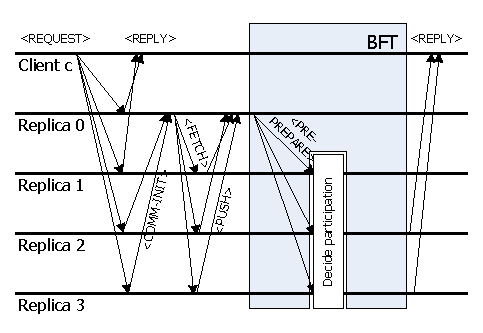
\includegraphics{Overview.eps}
\caption{A timeline view of the protocol, as a wrapper around BFT.}
\label{fig:overview}
\end{figure}

Figure~\ref{fig:overview} illustrates the structure of the consistency
protocol, and its relationship to BFT.

We use $\Re$ to denote the replica set, and integers $i \in \{0, \ldots,
|\Re|-1\}$ to denote individual replicas. Messages with a subscript of
the form $a_c$ denote a signature by principal $c$.  Malformed or
improperly signed messages are dropped without further processing.


\subsubsection{The Client}
A client $c$ with a request $o$ for the service multicasts the msssage
$<\msg{Req}, o, t, c>_{a_c}$ to all replicas, where $t$ is a local,
monotonically increasing timestamp.  It sets a timer and waits for replies to
its request from at least $2f+1$ replicas; a well formed reply has the
form $<\msg{Rep}, r, \mathit{CSN}, t, c, i>_{a_i}$, where $r$ is the
result of the reply according to replica $i$.  $\mathit{CSN} = <v,n>$
represents the current committed state of the service, and contains the
latest BFT view number $v$ and committed sequence number $n$.  The client
checks received replies for the request for matches on their $r$ and
$\mathit{CSN}$ fields.  Requests for
which the client has received no more than $2f$ matching replies are
\emph{submitted} while those for which the client has received at least
$2f+1$ matching replies are \emph{admitted}.

\Sys guarantees that reply values of admitted requests will lie within a
numerical error of $\alpha$ from the result of the request in its
eventual order in the replicated state machine's schedule.  Submitted
but not admitted requests \emph{may} eventually be committed, but no
guarantee is given on their reply value.  As soon as a request is
admitted (i.e., at least $2f+1$ matching replies have been collected),
the client returns the reply value $r$ up to the application.  If the
timer expires before the request is admitted, the client retransmits the
request.  A correct client has only a single request in flight at any
point in time.






\subsection{Replica Request Handling}

A service replica responds to client requests according to
Algorithm~\ref{alg:replicaReply}.  In addition to BFT state, the replica
holds a list $T$ of tentative updates it has received since the last BFT
commit, as well as an identifier $\mathit{CSN}$ for that commit
consisting of a BFT view number and sequence number. The replica also 
maintains the largest request timestamp it has processed for every
client, as well as a cache of recent reply messages sent.

\begin{algorithm}
\small
\caption{Algorithm to respond to a client request at replica $i$. }
On reception of $<\msg{Req}, o, t, c>_{a_c}$
\begin{algorithmic}[1]\label{alg:replicaReply}
\IF[If the new client timestamp is one greater that the last known for
the client and I can take more requests]{$(t = t_c+1) \wedge \neg \mathit{busy}$}
\STATE $\mathtt{boundError}(o, t, c, \beta)$ \COMMENT{May block here, if checkpoint is required.}
\STATE $r \leftarrow \mathtt{eval}(o, S, c)$ \COMMENT{Evaluate the
  request on last checkpoint state along with tentatives of the same
  client.}
  \label{lin:sendReply}
\STATE $T \leftarrow T \cup <o, t, c>$ \COMMENT{Append the request to my tentatives.}
\STATE $t_c \leftarrow t$ \COMMENT{Update latest timestamp remembered
  from the client.}
\STATE $\mathtt{cache}(<o, t, c>_{a_c}, <\msg{Rep}, r, \mathit{CSN}, t, c,
    i>_{a_i})$ \COMMENT{Cache the reply message in case the client
    retransmits the request.}
\STATE send $<\msg{Rep}, r, \mathit{CSN}, t, c, i>_{a_i}$ to $c$
\ELSE
\IF[Check if this is an old request with a cached reply.] {$t \in \mathit{replyCache}_c$}
\STATE send $\mathit{replyCacheMsg}_c^t$ to  $c$ \COMMENT{Send the
  cached reply message.}
\ELSIF [Store the request if more recent than last known] {$t > t_c$}
\STATE {$U \leftarrow U \cup <REQ, o, t, c>_{a_c}$} \COMMENT{Store in $U$, a buffer storing un-answered requests.}
\ENDIF
\ENDIF
\end{algorithmic}
\end{algorithm}

When it receives a client request, the replica checks if the timestamp
on that request is smaller than the remembered timestamp for the
client, indicating this is an old request retransmission. In that case,
a reply for that request is retransmitted to the client if it is still
cached but the stale request is not processed further.  If instead this
is a new request, the replica ensures it is not in danger of violating its
bounded consistency guarantees via the $\mathtt{boundError}$
function. It then evaluates the request on the latest service state $S$
it knows, producing a tentative result value $r$, stores the request in its
tentative list, and sends the client a reply with the tentative result.

Evaluation of a tentative request $o$ with regards to latest checkpoint
state $S$ is done by applying all prior tentative requests in $T$ by the same
client $c$ to that state, then applying $o$, and returning the result.
This ensures that the client receives ``read your writes'' session
guarantees on its own tentative requests between checkpoints.

The $\mathtt{boundError}$ function is presented in pseudocode in
Algorithm~\ref{alg:boundError}. If the inclusion of the new request $o$
into the replica's tentative updates causes neither the total
postive weight nor the total negative weight of tentative updates to
exceed a threshold $\beta$, then the function returns immediately.
Otherwise, the replica must ensure that all of its tentative updates are
committed before it can take on any more.  It begins the process by
sending a $\msg{ComInit}$ message to the current consistency
primary (for convenience, we use the BFT primary, but that is not
required), and blocks until all of its tentative updates have been
committed.  The $\msg{ComInit}$ message is retransmitted a
maximum number of times and as a last resort a BFT view change is
initiated when no checkpoint is committed, restarting the commit process
under a new primary.  We explain the workings of the consistency
protocol in the following section.

\begin{algorithm}
\small
\caption{Algorithm to bound numerical error.}
$\mathtt{boundError}(o, t, c, \beta)$
\begin{algorithmic}[1]\label{alg:boundError}
\IF [The new request causes either my positive- or negative-weight
  tentative updates to go over the commit threshold.] {$(|F(T_+ \cup <o,
  t, c>)| >
  \beta) \vee (|F(T_- \cup <o, t, c>)| > \beta)$}
\STATE $p \leftarrow \mathtt{bi.primary}$ \COMMENT{Find the BI's primary.}
\STATE send $<\msg{ComInit}, i, \mathit{CSN}>_{a_i}$ to $p$
  \COMMENT{Initiate a checkpoint commit with current tentative updates.}
\STATE \textbf{block} until $\mathtt{bft.execute}$ delivers
  a successfully committed checkpoint and retransmit up to $k$ times
\IF {Timeout}
\STATE $\mathtt{bi.primaryChange}()$ \COMMENT{Change the BI's primary.}
\ENDIF
\ENDIF
\end{algorithmic}
\end{algorithm}


\subsection{Consistency Protocol}
Once a replica has decided a checkpoint commit must occur, sending a
$\msg{ComInit}$ message to the primary, the consistency protocol is
started (Algorithm~\ref{alg:receiveComInit}).  First, the primary requests--via a $\msg{Fetch}$
message--tentative updates for the next checkpoint from all replicas,
which they return in $\msg{Push}$ messages (Algorithm~\ref{alg:receiveFetch}).
Once it has collected at least $2f$ distinct $\msg{Push}$ messages from
replicas with up-to-date checkpoint identifiers ($\mathit{CSN}$s, the
primary  eliminates duplicate tentative updates and combines what
remains into the next batch of updates for commit.  It submits
these updates to the BFT protocol as a single BFT request via the
$\mathtt{bft.invoke}$ interface function (Algorithm~\ref{alg:receivePush}).
The request to the BFT protocol is constructed by putting a quorum of 
$\msg{Push}$ messages. This is important to ensure that a quorum of replicas
can validate that the request to the BFT was in fact constructed by a 
quorum of valid $\msg{Push}$ messages and hence safe to execute the requests
contained since it is guaranteed to contain every admitted update since last
committed checkpoint. Proof is provided in Section~\ref{sec:analysis}.

\begin{algorithm}
\small
\caption{Message handler for $\msg{ComInit}$ messages at replica $i$.}
On reception of $<\msg{ComInit}, j, \mathit{CSN}_j>_{a_j}$
\begin{algorithmic}[1]\label{alg:receiveComInit}
\IF [Am I the primary, am I free, and are we on the same checkpoint?]
    {$(i = \mathtt{bi.primary}) \wedge
      \neg \mathit{busy} \wedge
      (\mathit{CSN}_j = \mathit{CSN})$}
\STATE $\mathit{busy} \leftarrow \mathtt{true}$
\STATE $\mathit{pushMsgs}_{\mathit{CSN}.n+1} \leftarrow
\{<\msg{Push}, T, \mathit{CSN}, i>_{a_i}\}$
\STATE multicast $<\msg{Fetch}, \mathit{CSN}.n + 1, i>_{a_i}$
\ENDIF
\end{algorithmic}
\end{algorithm}


\begin{algorithm}
\small
\caption{Message handler for $\msg{Fetch}$ messages at replica $i$.}
On reception of $<\msg{Fetch}, n, j>_{a_j}$
\begin{algorithmic}[1]\label{alg:receiveFetch}
\IF [Is sender the primary? Is this the next sequence number?]
    {$(j = \mathtt{bi.primary}) \wedge (n = \mathit{CSN}.n+1)$}
\STATE send $<\msg{Push}, T, n, i>_{a_i}$ to $p$
\ENDIF
\end{algorithmic}
\end{algorithm}


\begin{algorithm}
\small
\caption{Message handler for $\msg{Push}$ messages at replica $i$.}
On reception of $m \leftarrow <\msg{Push}, T', n, j>_{a_j}$
\begin{algorithmic}[1]\label{alg:receivePush}
\IF [Am I the primary and engaged in a checkpoint?]
    {$(i = \mathtt{bft.primary}) \wedge \mathit{busy}$}
\IF [Is this a valid update list?]
    {$(|F(T'_+)| \leq \beta) \wedge (|F(T'_-)| \leq \beta) \wedge (n = \mathit{CSN}.n + 1)$}
\STATE $\mathit{pushMsgs}_{\mathit{CSN}.n+1} \leftarrow
\mathit{pushMsgs}_{\mathit{CSN}.n+1} \cup m$
\IF [Have I got enough $\msg{Push}$ messages?]
    {$|\mathit{pushMsgs}_{\mathit{CSN}.n+1}| \ge (2f+1)$}
\STATE $T_\mathit{prop} \leftarrow \{l.T | l \in
    \mathit{pushMsgs}_{\mathit{CSN}.n+1}\}$ \COMMENT{Combine tentative
    update lists, ordering according to client id, client timestamp.}\label{lin:combinePushOrdering}
\STATE $\mathtt{bft.invoke}(T_\mathit{prop})$ \COMMENT{Run BFT on batch update.}
       \label{lin:bftInvoke}
\ENDIF
\ENDIF
\ENDIF
\end{algorithmic}
\end{algorithm}

\if 0
\subsection{Interface to BFT}

The active interaction of the consistency protocol with BFT occurs on
four occasions: (a) the submission of a new update batch via
$\mathtt{bft.invoke}$ (Algorithm~\ref{alg:receivePush} in the previous section), (b) the
interception and conditional forwarding of a $\msg{PrePrepare}$ message
(Algorithm~\ref{alg:receivePrePrepare}), (c) the receipt of a commit
notification via $\mathtt{bft.execute}$
(Algorithm~\ref{alg:execute}), and (d) the initiation of BFT view
change (Algorithm~\ref{alg:boundError}). \note{This would be a good place to use, instead,
the BFT client interface, removing all connection to the innards of
BFT.  Can we cast the whole thing as if we're controlling what the
application sends and receives from the BFT client proxy?}

Interception of $\msg{PrePrepare}$ messages allows a replica to validate
the update batch submitted to BFT by the primary. Validation includes
checking that no request in the batch may receive an eventual result
that is numerically different by more than $\alpha$ from what it may
have received tentatively, and that no request in the validating
replica's tentative update list has been excluded.  Failed validation
causes the replica to drop the $\msg{PrePrepare}$ message.

\begin{algorithm}
\small
\caption{Intercept handler for $\msg{PrePrepare}$ messages. It validates
 the content of the message--that is, the batched tentative updates
 being committed--and only delivers it to BFT if it is valid.}
On reception of $<\msg{PrePrepare}, v, n, d>$
\begin{algorithmic}[1]\label{alg:receivePrePrepare}
\IF [I do not have a proposed update for this $\msg{PrePrepare}$
    message.]
    {$(\not \exists T' = m.T | (m \in \mathtt{bft.in} \wedge m =
      <\msg{REQUEST}, T, \mathit{ts}, \mathit{cl}> ) )$}
    \STATE \textbf{drop}
\ELSIF [BFT round does not correspond to the next checkpoint.]
	{$(n \neq \mathit{CSN}.n + 1)$}
	\STATE \textbf{drop}
\ELSIF [Proposed batch violates error bounds.]
       {$(|F(T'_+)| > \alpha) \vee (|F(T'_-)| > \alpha)$}
	\label{lin:maxPrePrepareBatchWeight}
	\STATE \textbf{drop}
\ELSIF [My tentative updates are not included in the proposed update.]
       {$T \not \subseteq T_\mathit{prop}$}
       \label{lin:updateInclusion}
       \STATE \textbf{drop}
\ELSIF [Some updates by the same client are not ordered by timestamp.]
       {$\exists 0 \leq i < j \leq (|T|-1) |
	 T[i].c = T[j].c \wedge
	 T[i].t \geq T[j].t$}
	\label{lin:clientUpdateOrdering}
	\STATE \textbf{drop}
\ELSE
\STATE $\mathit{busy} \leftarrow \mathtt{true}$ \COMMENT{Now I'm
  involved in a checkpoint.}
\STATE \textbf{pass through} $m$ \COMMENT{Let BFT have the message.}
\ENDIF
\end{algorithmic}
\end{algorithm}

\fi

\subsection{Validation}
When BFT ultimately commits a batch update, a replica receives a
$\mathtt{bft.execute}$ callback. Algorithm~\ref{alg:execute} describes
how replicas update their state once a checkpoint has been committed.
Each non-faulty replica needs to validate the checkpoint that committed, i.e.,
whether it contains at least $2f+1$ valid $\msg{Push}$ messages, numerical weight
of the updates does not exceed $\alpha$ and whether it is able to order them 
correctly. If any of these conditions does not satisfy, then the checkpoint is
dropped, which will eventually trigger a BFT view change since primary is faulty
(correctness is proved in Section~\ref{sec:analysis}. If valid,
the checkpoint identifier is advanced to the latest committed one, the
committed service state at the replica is updated with the 
update batch, all per-client state is updated as per the committed
updates, and any committed updates in the tentative list are
removed. For every committed update, the replica constructs a reply
message and inserts it into its local cache, in case a client
retransmits the request.

One point to note is that to verify whether there are $2f+1$ valid $\msg{Push}$
messages are present in a checkpoint, these $\msg{Push}$ messages need to be 
signed via asymmetric cryptography (i.e., using pub/priv key pair). Moreover, the
requests contained in the $\msg{Push}$ messages should also be signed by clients
using their private keys. Since client side cryptographic overhead is not the 
bottleneck, this is not a concern. Moroever, we believe that signing the $\msg{Push}$ message
with asymmetric crypto will not incur huge overhead since it is done once per checkpoint
,avoids the bad authenticators faulty replicas may send and the cost of encryption continues
to drop (with 512 bit keys, can be completed in sub-milliseconds). Finally, using authenticators
typically adds another round trip and in high delay environments, signing is a better tradeoff.
We therefore leave the
use of MACs and authenticators for the $\msg{Push}$ messages for future work. Note that
the BFT protocol is left unchanged in this respect and it continues to use authenticators and MACs.
\begin{algorithm}
\small
\caption{Upcall from BFT once an update batch $T'$ is committed in view
  $v$ with sequence number $n$.}
$\mathtt{execute}(T', v, n)$
\begin{algorithmic}[1]\label{alg:execute}
\STATE $\mathit{CSN} \leftarrow <v, n + 1>$
\IF [Not enough valid $\msg{Push}$ messages in the checkpoint?]
    {$|\mathtt{T'.pushMsgs}| < 2f+1$}
    \label{lin:checkQuorumPush}
\STATE \textbf{drop}
\ENDIF
\IF [[Proposed batch violates error bounds.]
       {$(|F(T'_+)| > \alpha) \vee (|F(T'_-)| > \alpha)$}
        \label{lin:maxPrePrepareBatchWeight}
        \STATE \textbf{drop}
\ENDIF
\STATE $\mathtt{l = order(T'.pushMsgs)}$ \COMMENT{Construct an ordering of 
requests contained in $\msg{PushMsg}$'s in $T'$, 
based on client id and timestamp, duplicates removed.}
\label{lin:constructOrdering}
\FORALL {$<o, t, c>_{a_c} \in \mathtt{l}$}
\STATE $r \leftarrow \mathtt{eval}(o, S)$ \COMMENT{Evaluate the
  request on the stable service state, update the state.}
  \label{lin:evaluateCommitted}
\STATE $\mathtt{cache}(<o, t, c>_{a_c}, <\msg{Rep}, r, \mathit{CSN}, t, c,
    i>_{a_i})$ \COMMENT{Cache the reply message in case the client
    retransmits the request.}
%\STATE $S \leftarrow \mathtt{apply}(S, o)$ \COMMENT{Update local state
    %with update.}
\ENDFOR
\STATE $T \leftarrow T \setminus \mathtt{l}$ \COMMENT{Remove committed updates from my
    list of tentatives.}
\STATE $\mathit{busy} \leftarrow \mathtt{false}$
\end{algorithmic}
\end{algorithm}



\subsection{Extensions}

This section deals with aspects of \Sys that have no bearing on its
safety, but can improve its performance, such as dealing with overload, thwarting
``trigger-happy'' faulty replicas that invoke frivolous checkpoint
commitments, and catch-up for slow replicas.

\if 0
\subsubsection{Eliminate Spurrious Client Retransmits}
\note{Does this need to be an optimization? We can probably put it in
  the basic protocol.}
The basic version of the protocol drops all requests that arrive at a
replica while that replica is participating in the consistency or
consensus protocol. Clients who happen to send a request at that time
must timeout before retransmitting their request.

A simple optimization allows replicas to queue requests without
responding while busy, and process them once free again.

\fi

\subsubsection{High Request Rates}
When request rates are high, the basic version of \Sys becomes
BFT-bound, moving from checkpoint to checkpoint at a rate of $k$
requests per checkpoint, where $\beta \leq k \leq \alpha$.  Since request queues at
replicas ``drain'' at this rate, if request arrival rate is greater than
$k$ per checkpoint duration, the system will overflow.

A useful optimization is to allow the system to ``drain'' request queues
faster, by allowing a \emph{hybrid} batch of updates to commit in a
single BFT invocation.  Specifically, when a replica completes a
checkpoint and finds its request queue containing more than
$\beta$-weighted updates, it processes the first $\beta$-weighted
updates as usual (i.e., replying to clients with tentative results) and
holds on to the remainder of its queue. During the consistency protocol,
the client sends a $\msg{Push}$ message that contains not only its
tentatively answered updates, but also all queued requests as well, in a
separate request list.  The primary proposes an update batch made of all
tentatively answered updates first, followed by all unanswered, queued
requests from all replicas; it is important that tentative updates are
first in the proposed update sequence, to ensure they remain within the
error bounds, and validation in Algorithm~\ref{alg:receivePrePrepare} must also
check this condition.  Once the commit is completed, replicas give
definitive (that is, consistent with committed state) replies to all
unanswered, queued requests to corresponding clients, thereby
``draining'' their queues at a rate greater than what the
bounded-consistency protocol alone allows.


\subsubsection{Commit-Rate Lower Bound}

The basic algorithm ensures that the safety condition is met, i.e., that
BFT is executed frequently enough so that no result to a tentative
update experiences more than a maximum numerical error.  However,
nothing stops the faulty replicas from inducing more frequent BFT rounds
than necessary, e.g., by sending spurrious $\msg{ComInit}$ messages.

We can modify Algorithm~\ref{alg:receiveComInit} to wait for at least
$f+1$ $\msg{ComInit}$ messages from different replicas before sending a
$\msg{Fetch}$ message.  In this fashion, BFT invocations will only occur
when at least one current replica has legitimately reached its bound of
tentative updates.

This solution does not prevent traditional denial-of-service attacks, in
which malicious clients send spurrious requests at a high rate.
\Sys remains vulnerable to such attacks, similarly to its precursor
systems, and can mitigate their effects via typical DoS counter measures
such as request rate limits.


\subsubsection{Catch-up for Slow Replicas}

As with the original BFT protocol, special care is needed to ensure slow
replicas can catch up with the latest state of the system. Although not
present in the protocol description above, we leverage the state
transfer mechanisms employed by BFT for the same purpose to bring
lagging replicas up to date even with regards to the state of the
consistency protocol.


\subsubsection{Large Batch Sizes}

As the inconsistency bound grows, or, equivalently, the request rate
grows, the system will have to commit larger batches of updates.  Past a
batch size, minimizing the number of BFT rounds has diminishing returns
due to the cost of transmitting large requests.  It is preferable in
those cases to break down a large batch of updates into multiple
smaller ones, taking advantage of BFT's inherent pipelining.    For
those cases, we can increase BFT's high-water-mark to allow multiple BFT
rounds in flight.  Replicas need not reject update batches that do not
contain all their local tentative updates; however, they do need to wait
until all their tentative updates have been included in an update batch
before processing more requests from their queues.
























































































\section{Analysis}
\label{sec:analysis}

In this section we prove informally the consistency guarantees of \Sys. The
\emph{safety} guarantee of \Sys is, informally, that every tentative
reply to an \emph{admitted} request will contain a result that lies
within numerical error bound $\alpha$ from the result of that same
request in its committed order.  The \emph{liveness} guarantee of \Sys
is  that non-faulty
replicas do not wait indefinitely to commit their local tentative updates.

\subsection{Safety}
We first start with some basic definitions.

\subsubsection{Definitions}

We need to first define what is a strictly consistent history is and what
is the history seen by a tentative response. Then we have to define the
numerical weight seen by a response.

\textbf{Definition 1}: A history, $GH$, consisting of all
requests processed by the system is \emph{linearizable} if it is sequential and 
compatible with external ordering. This is the strongest form of consistency.

\textbf{Definition 2}: A history, $CH$, consisting of all requests \emph{committed}
by the state machine replication BFT protocol is linearizable. 

\textbf{Definition 3}: A history, $TH$, consisting of a prefix of the $CH$ plus a set
of tentative requests is called the \emph{tentative history}. Only the tentative requests can
be re-ordered when they appear in $CH$. A non-faulty replica's local history is a tentative
history.

\textbf{Definition 4}: Given a history $H=\{\mathtt{w_1,w_2,w_3...,w_k}\}$, the numerical
weight NW of $H$ is given by NW($H$)= $F(H) = F(\mathtt{w_1,w_2,w_3..,w_k}) = F(\mathtt{w_1})+
F(\mathtt{w_2})+...+F(\mathtt{w_k})$.

\textbf{Definition 5}:
Numerical error between a tentative response $r$ and
committed response $r'$ to a request $o$ is given by the absolute difference between
the NW of the prefix of $TH$ seen by $r$ and the NW of the prefix of $CH$ seen by $r'$.


\textbf{Definition 6}: A set of updates $U=\{\mathtt{o_1,o_2,..,o_k}\}$, where 
each $\mathtt{o_i}$ is a request, is \emph{$<$clientId, seq$>$-ordered} if following holds:\\
$\forall \mathtt{o_i, o_j \in U: o_i < o_j}$ if 
\begin{itemize}
\item{} $\mathtt{o_i.clientId < o_j.clientId}$ (clientId of a request represents
the numerical identifier of the client).
\item{} $\mathtt{o_i.clientId == o_j.clientId \wedge o_i.{seq} < o_j.{seq}}$ 
($\mathtt{o_i.{seq}}$ is the sequence number assigned by the client to a request).
\end{itemize} 

%Note that an \emph{$<$clientId, seq$>$-ordered} set of updates is totally ordered. This is important
%since it allows non-faulty replicas to agree on the same ordering of updates given that
%each non-faulty replica uses the same set of updates to determine the ordering.

\textbf{Definition 7}: A checkpoint $C^i=\{\mathtt{o_1,o_2,..,o_k}\}$, where 
$\mathtt{o}$ is a request, is valid if
% = \{\mathtt{<T_i><T_{i+1}>...<T_{i+2f+1}>}\}$, where 
%$\mathtt{T_i}$ represents the requests sent by replica $i$ in $\msg{Push}$ message, is 

\begin{enumerate}
\item{} it contains every admitted 
request after the previous valid checkpoint $C^{i-1}$.
\item{}  $(|F(C^{i}_+)| \leq \alpha) \wedge
(|F(C^{i}_-)| \leq \alpha)$.
%\item{} $C^i$ is \emph{$<$clientId, seq$>$-ordered}.
\item{}if $C^i_j$ is the subset of $C^i$ containing requests only from client $j$, then
$\forall o_1, o_2 \in C^i_j, o_1 < o_2 \implies o_1.seq < o_2.seq$.
%the requests in $C^i_j$ are ordered by the sequence number assigned by the client $j$. 
This implies that requests from a given client appear in the order assigned by the client.
\end{enumerate}
%\end{def}


\textbf{Definition 8}: A $\msg{Push}$ message $\mathtt{P}$ from replica $R$ for checkpoint $C^i$ is valid if
\begin{itemize}
\item{} $(|F(P_-)| \leq \beta) \wedge (F(P_+) \leq \beta)$.
\item{} Includes every request replica $R$ locally received after checkpoint $C^{i-1}$.
%\item{} $\mathtt{P}$ is \emph{$<$clientId, seq$>$-ordered}.
%requests from same client in $\mathtt{P}$ are ordered according to the
%timestamp.
\end{itemize}

\textbf{Definition 9}: A checkpoint $C$ executes if all admitted updates contained in $C$ are 
executed correctly by at least $f+1$ non-faulty replicas.

We will show that the checkpoint constructed by our algorithm in a non-faulty
execution is a valid checkpoint and that a valid checkpoint will be eventually
committed and executed. 

\subsubsection{Proofs}

\begin{theorem}[Valid Checkpoints]
\label{thm:validCheckpoints}
A checkpoint executes if and only if it is valid.
\end{theorem}



We start by showing that every admitted request is included in the next
checkpoint.
 
\begin{lemma}
\label{lem:admittedUpdatesInNextCheckpoint}
Union of requests present in the valid $\msg{Push}$ messages from at least $2f+1$
non-faulty replicas for
checkpoint $C^i$ contains every admitted request after checkpoint $C^{i-1}$.
%The $i$-th checkpoint contains every admitted request after $i-1$-st checkpoint
%if it includes every request from at least $2f+1$ valid $\msg{Push}$ messages.
\end{lemma}
\begin{proof}
Let $o$ be a request admitted after the $i-1$-st
checkpoint.
From the
definition of admission, the client has received at least $2f+1$ matching replies
to request $o$ from a subset $P$ of replicas ($|P| \geq 2f+1$) , of
which at least $f+1$ are non-faulty
replicas. Therefore, request $o$ appears in the $\msg{Push}$ message of at least
$f+1$ non-faulty replicas. 
%ed in the tentative update list
%after checkpoint $i-1$ of at least those $f+1$ non-faulty replicas.

Any two quorums of $2f+1$ replicas intersect in at least $f+1$ replicas, 
at least one being non-faulty. Therefore, union of $\msg{Push}$ messages from
a quorum of $2f+1$ replicas for checkpoint $C^i$ ensures that request $o$ appears in
it since at least one non-faulty replica's $\msg{Push}$ message contains it. Since this 
holds for every admitted request, union of any quorum of $2f+1$ $\msg{Push}$ 
messages contains every admitted request after checkpoint $C^{i-1}$.
%The $i$-th checkpoint is constructed by taking the union of the tentative requests
%By taking union of valid $\msg{Push}$ from a subset $Q$ of the replicas ($|Q| \geq 2f+1$), at least $f+1$ of them
%are non-faulty. By the quorum intersection property ($P$ and $Q$ have at least
%$f+1$ non-faulty replicas common), each admitted request after the $i-1$-st 
%checkpoint will appear in the tentative requests of at least one non-faulty 
%replica in $Q$
%and therefore appear in $i$-th checkpoint.  
%ch. Hence, request $o$ will appear in the checkpoint.
\if 0

By taking union of the updates from $2f+1$ replicas, it is guaranteed that at
least $f+1$ non-faulty replicas 


For the successful commitment of the $i$-th checkpoint, at least a
subset $Q$ of replicas ($|Q| \geq 2f+1$)
must have completed BFT and, therefore, passed validation at
Line~\ref{lin:updateInclusion} of
Algorithm~\ref{alg:receivePrePrepare}. Therefore, all replicas in $Q$
must have ensured their tentative updates after checkpoint
$i-1$ are included in the committed batch at checkpoint $i$.

The two subsets $P$ and $Q$ must overlap in at least $f+1$ nodes (since
the total population contains $3f+1$ replicas), of which at least one is
non-faulty. As a result, request $o$ must be in the $i$-th checkpoint.
\fi
\end{proof}

\if 0
\begin{lemma}
\label{lem:admittedCheckpoint}
Any committed checkpoint $C$ must contain every admitted request after the last
committed checkpoint.
\end{lemma}
\begin{proof}
For the successful commitment of the $i$-th checkpoint, at least a
subset $Q$ of replicas ($|Q| \geq 2f+1$)
must have completed BFT and, therefore, passed validation at
Line~\ref{lin:updateInclusion} of
Algorithm~\ref{alg:receivePrePrepare}. Therefore, all replicas in $Q$
must have ensured their tentative updates after checkpoint
$i-1$ are included in the checkpoint $i$.
Lemma~\ref{lem:admittedUpdatesInNextCheckpoint} ensures that such a checkpoint
contains all requests that are admitted after the last committed checkpoint.
\end{proof}


\begin{lemma}
\label{lem:maxCheckpointWeight}
Any committed checkpoint $C$ must satisfy $(|F(C_+)| \leq \alpha) \wedge
(|F(C_-)| \leq \alpha)$.
\end{lemma}
\begin{proof}
Algorithm~\ref{alg:receivePrePrepare} ensures at
Line~\ref{lin:maxPrePrepareBatchWeight} that no non-faulty replica will
participate in a checkpoint commitment that contains updates that
violate the above conditions. That guarantees that no such checkpoint
will be committed, since BFT will not be invoked at any non-faulty
replicas for it. One can rephrase the above arguement as follows: for every
checkpoint that eventually commits, the above condition is satisfied.
\end{proof}

Note that the above Lemma does not imply that every checkpoint that satisfies
the above condition will always commit.

\begin{lemma}
\label{lem:validCheckpoint}
Every committed checkpoint is a valid checkpoint.
\end{lemma}
\begin{proof}
Follows directly from Lemma~\ref{lem:admittedCheckpoint} and 
Lemma~\ref{lem:maxCheckpointWeight}.
\end{proof}
\fi


\begin{lemma}
\label{lem:validPush}
If $U$ contains union of requests in $2f+1$ valid $\msg{Push}$ messages, then
$(F(U_+) \leq \alpha) \wedge (|F(U_-)| \leq \alpha)$.
%ensures that
%\begin{itemize}
%\item{} $(F(C_+) \leq \alpha) \wedge (|F(C_-)| \leq \alpha)$.
%\item{} Preserves ordering among the requests from the same client according to
%the timestamp assigned by the client.
%\end{itemize}
\end{lemma}
\begin{proof}
By definition, a non-faulty replica only sends a valid $\msg{Push}$ message. By 
waiting for at least $2f+1$ valid $\msg{Push}$ messages and setting 
$\beta =\alpha/(3f+1)$, we have 
$F(U_+) = (2f+1).\beta = (2f+1).\alpha/(3f+1) \leq \alpha$. Similarly, $|F(U_-)| \leq \alpha$. Note 
that a replica that sends an invalid $\msg{Push}$ message is not included and it 
is safe to wait for another $\msg{Push}$ message since a non-faulty replica never
sends an invalid $\msg{Push}$ message.
\if 0
Line~\ref{lin:combinePushOrdering} of Algorithm~\ref{alg:receivePush} orders the
requests contained in the $\msg{Push}$ messages according to client id and the
timestamp assigned to the request by the client. This is a deterministic ordering
which ensures that requests from a given client are ordered according to the
timestamps assigned by the client. If the client is non-faulty, it will always
assign a monotonically increasing timestamp to its requests. A faulty client may
submit two different requests at the same timestamp at two different replicas. 
We pick one at random since none of them is guaranteed to be an admitted request.
A non-faulty who has a different request  for the same client timestamp would 
conclude that only a faulty client can submit two different request at the same
timestamp and hence would accept the one contained in the checkpoint.
\fi
\end{proof}


\begin{lemma}
A checkpoint constructed by taking the union of requests contained 
in $2f+1$ valid $\msg{Push}$ messages and ordered according to \emph{$<$clientId, seq$>$-ordering}
is a valid checkpoint.
\end{lemma}
\begin{proof}
Follows directly from Lemma~\ref{lem:admittedUpdatesInNextCheckpoint} and 
Lemma~\ref{lem:validPush} and the fact that \emph{$<$clientId, seq$>$-ordering} 
produces a total ordering of a set of requests which satisfies the partial ordering
required by the 3rd condition of a valid checkpoint. To see that, note that under 
\emph{$<$clientId, seq$>$-ordering}, requests from same client are ordered according
to the client generated sequence number. 
\end{proof}

Now, we can prove  Theorem~\ref{thm:validCheckpoints}.

\begin{proof}
We need to prove two cases: (i)
every executed checkpoint is a valid checkpoint and (ii) every valid checkpoint
eventually executes.

Case (i). By contradiction. Let $C$ be a checkpoint that executes and
that it is an invalid checkpoint. 
A checkpoint is invalid if either it misses an admitted update or 
contains more than $\alpha$-weighted updates or some updates from a client are not
ordered correctly. $C$ may miss some admitted upates if it is constructed out of
less than $2f+1$ valid $\msg{Push}$ messages from distinct replicas. Line ~\ref{lin:checkQuorumPush}
in 
Algorithm~\ref{alg:execute} ensures that no non-faulty replicas executes a checkpoint if 
it does not contain $2f+1$ valid $\msg{Push}$ messages and therefore not executed, 
a contradiction. An invalid checkpoint may contain more than $\alpha$-weighted updates, 
which no non-faulty replica would allow to execute as per Line
~\ref{lin:maxPrePrepareBatchWeight} in Algorithm~\ref{alg:execute}, another contradiction. 
At Line ~\ref{lin:constructOrdering} in 
Algorithm~\ref{alg:execute}, at least $f+1$ non-faulty replicas would construct a deterministic 
\emph{$<$clientId, seq$>$-ordering} of updates. Since BFT ensures that each such replica receives the identical 
checkpoint, each one of them would produce the same ordering. If unable to order, 
none of these non-faulty replicas would execute the checkpoint, yielding another contradiction.



Case (ii). Consider a valid checkpoint that is passed to the BFT protocol at Line 
~\ref{lin:bftInvoke} in Algorithm~\ref{alg:receivePush}. 
At least $f+1$ non-faulty replicas would get an $\mathtt{execute}$ 
upcall, Algorithm~\ref{alg:execute}, with identical valid checkpoint $T'$. Since $T'$ is valid, at 
least these many non-faulty replicas would pass the test at Line~\ref{lin:checkQuorumPush} 
and Line~\ref{lin:maxPrePrepareBatchWeight}. 
Moreover, since $T'$ is identical in these many replicas, the \emph{$<$clientId, seq$>$-ordering} produces 
a consistent $\mathtt{l}$ at these replicas. Once that happens, at least $f+1$ such non-faulty 
replicas would execute the admitted requests and hence execute the checkpoint. 

\end{proof}

%Lemma~\ref{lem:admittedUpdatesInNextCheckpoint} and
%\ref{lem:maxCheckpointWeight} together guarantee that every admitted
%update, once committed, appears in a checkpoint $U$ that bounds the
%total weight of included updates by $\alpha$.  

Now, given that only valid checkpoints can execute,  
we can proceed to
prove the following safety theorem.

\begin{theorem}[Safety]
\label{thm:safety}
For every admitted and subsequently committed and executed request $o$, the result
$r$ produced when the request is executed in a non-faulty replica at
Line~\ref{lin:evaluateCommitted} of Algorithm~\ref{alg:execute} and the
result $r'$ matching $2f+1$ tentative replies sent in
Line~\ref{lin:sendReply} of Algorithm~\ref{alg:replicaReply} it is guaranteed 
that the numerical error between $r$ and $r'$ is bounded by $\alpha$.
%$|r-r'| \leq \alpha$.
\end{theorem}

\begin{proof}
Note that the history produced by checkpoints is a linearizable history (follows
from definition). To prove the theorem, we have to show that the history 
seen by a tentative response and a committed response (a response prepared when this requests appears 
in a checkpoint) to an admitted request can
not differ by more than $\alpha$.

Let $U$ denote the sequence of admitted updates by the same client
preceding $o$ at a non-faulty replying replica's tentative updates
list. Since $o$ is admitted, at least $f+1$ non-faulty replicas have consistent
$U$.
The history $H_o^{C^{i-1}}$ of updates seen by $o$ consists of every update executed and committed till
checkpoint $C^{i-1}$ plus the updates in $U$. So, the weight of updates
seen by result $r$ to request $o$ is given by $F(H_o^{C^{i-1}}) = F(H^{C^{i-1}}) + F(U)$.


\if 0
No checkpoint can commit in which updates by the same client are
not ordered by their client assigned sequence numbers, and therefore differently from $U$,
because of Algorithm~\ref{alg:receivePrePrepare},
Line~\ref{lin:clientUpdateOrdering}. Algorithm~\ref{alg:replicaReply},
Line~\ref{lin:sendReply} specifies that a non-faulty replica first creates
a client specific state $S'$ by applying $U$ on the previous checkpoint state
$S$ and then applies the request $o$ to state $S'$. The
result $r_0$ for $o$ under an ordering $T_0$ in which $U$ and $o$ are
the first updates would be $r_0 = \mathtt{eval(o, S, U)}$, where
the weight of updates seen by $r_0$ is given by $F(H^o) = F(S + U) = F(S) + F(U) = F(S')$,
where $S$ is the application sate of the previous checkpoint and $S'$ is the current client 
specific application state.
\fi

Updates in the next valid checkpoint $C^i$ are \emph{$<$clientId, seq$>$-ordered}. Such an ordering
can be depicted as $C^i = c_0.c_1.c_2...c_k$, where $c_i$ represents the updates
submitted by client $i$ and assuming that there are at most $k$ clients.
Let $o$ be submitted by client $j$. So, the history seen by $o$, when 
when it appears in $C^i$ (Lemma 1) 
is the longest prefix of $C^i$ not containing $o$. This prefix $C^i_{prefix} =
c_0.c_1...c_j^{o.seq-1}$, where $c_j^{o.seq-1}$ represents the prefix of the updates submitted
by client $j$ not containing $o$. Note that $c_j^{o.seq-1}$ contains precisely the updates contained in $U$. Now,
the weight of result $r'$ produced when committed in checkpoint $C^i$ is given by $F(H^{C^{i-1}})+F(C^i_{prefix})$.

So, the numerical error seen by $o$ is difference of weight of histories seen by results $r$ and $r'$, denoted as
$|F(H^{C^{i-1}}) + F(C^i_{prefix}) - F(H_o^{C^{i-1}})|$.
On substituing for $F(H_o^{C^{i-1}})$, 
the numerical error is given by $|F(C^i_{prefix}) - F(U)|$. Since $U=c_j^{o.seq-1}$, 
the numerical error is now $|F(c_0.c_1...c_{j-1})|$. Since $C^i$ is a valid checkpoint, $F(C^i_+) \leq \alpha$.
This means that at worst, the weight of $F(c_0.c_1..c_{j-1})$ can be $\alpha$ which happens when 
every positive weight update from every other client gets a slot in front of $o$. Hence, the numerical
error seen by $o$ between response $r$ and $r'$ is bounded by $\alpha$. Similar argument applies when
all negative weighed updates are placed in front of $o$. 


\if 0
Any ordering $T$ for the eventual commitment of the checkpoint update
set $CU$ can be obtained from $T_0$ via a sequence of swaps of adjacent
updates.  Orderings that differ in a single such swap are themselves
\emph{adjacent}. Between adjacent orderings, $o$'s result value changes
only if $o$ is itself involved in an update swap; if $o$ swaps with its
successor update $s$, its result increases by $F(s)$ (note that $F(s)$
may be negative which will result in an absolute decrease in $o$'s
result). 

The value of $r_0$ can strictly increase via a sequence of
adjacent transformations in which, when $o$ is involved in a swap, its result
value increases in absolute. Starting with $T_0$, the only such swap
would be with a positive-weight successor, leaving a positive-weight
update preceding $o$ and all the rest following it in the
ordering. Recall that $o$'s predecessors in $T_0$ are updates in $C$
which cannot be reordered with regards to $o$. It
is easy to prove inductively that subsequent adjacent tranformations that strictly
increase $o$'s result value can only be swaps with other positive-weight
successors, and there can be no more than a $\alpha$-weight total increase in
$o$'s result value in such a sequence of strictly increasing-value
transformations, since $|F(CU_+)| \leq \alpha$. Similarly, via swaps with
negative-weight successors, $o$'s result value can at worst decrease by
$|F(CU_-)| \leq \alpha$.  Therefore, in any committed checkpoint, the result $r'$ of
$o$'s execution satisfies $|r-r'| \leq \alpha$.
\fi
\end{proof}




\subsection{Liveness}
For liveness, informally, we need to ensure that non-faulty
replicas do not wait indefinitely to commit their local tentative updates. 
First, note that the BFT protocol is live, meaning that if a checkpoint is
passed to the BFT protocol, then the protocol will eventually complete. To ensure
that the \Sys protocol is live given that the BFT protocol is live, we need to show 
that eventually a valid checkpoint is passed to the BFT protocol.

We have two cases to handle. First, a faulty primary at the consistency layer may 
simply reject the $\msg{Push}$ or $\msg{ComInit}$ messages and not submit the checkpoint request
to the BFT layer. Second, it may submit an invalid checkpoint in the 
request to the BFT layer. Both these cases occur only when the primary at the 
consistency layer is faulty. At a high level, we need to initiate a primary change
at the consistency layer when enough non-faulty replicas suspect the primary.

The primary at the consistency layer is conceptually different from the primary of the
BFT protocol. However, to avoid reinventing the wheel for changing the primary, we reuse the
primary change protocol of the BFT (called a view change protocol) and for that we require that the primary at 
the consistency layer and the BFT layer are the same. However, we need to ensure that
the primary does not have any additional \Sys protocol specific state that needs to be moved to the new
primary since otherwise we may need to extend the view change protocol. 
Fortunately, at the \Sys layer, the primary simply
collects $2f+1$ valid $\msg{Push}$ messages and assign it a 
sequence number one greater than the sequence number of the last checkpoint (which is obtained
by reading the last sequence number committed in the BFT protocol layer). View change protocol at the BFT layer ensures that the
new primary obtains the necessary BFT protocol information from the previous primary. Hence, \Sys 
can safely leverage the view change protocol of the BFT to handle faults of the primary at the consistency
layer.

Now, we illustrate the modification to the basic \Sys protocol to handle a faulty primary.
After sending either a $\msg{ComInit}$ or a $\msg{Push}$ to the primary, each 
non-faulty replica $r$ starts a timer T. If T expires before the replica gets the 
$\mathtt{execute}$ upcall from the BFT layer, it multicasts its tentative updates 
to other replicas and restarts the timer again. If T expires again this time, it
requests a view change from the 
BFT layer. Or if the checkpoint contained in the $\mathtt{execute}$ upcall is not
valid, again a view change is requested. This is similar to the HQ protocol where
the primary is needed to collect the conflict certificates to submit to the BFT protocol
and a faulty primary is dealt by requesting a view change from the BFT protocol.

Now, we informally argue that \Sys is live.

First, note that if the primary is non-faulty, \Sys is live. 

Now,  consider  a faulty  primary.  Suppose that a non-faulty replica $r$ sends a $\msg{ComInit}$
message to the primary since it has received a batch of $\beta$-weighted requests. The primary
may simply  drop  the $\msg{ComInit}$ or $\msg{Push}$ 
messages. Replica $r$'s timer T will timeout and it will propagate its updates to
other replicas and restart timer T.  This propagation of updates ensures that at
least  f other non-faulty  replicas will  also see  these tentative  updates. At
least these many non-faulty replicas will  then wait for the BFT layer to provide the
$\mathtt{execute}$ upcall. If they timeout, at least $f+1$ non-faulty replicas will initiate a view
change  and this  time,  they will  successfully  change the  primary. If an invalid 
checkpoint is present in the $\mathtt{execute}$ upcall, then again no non-faulty
replica would execute it and again request a view change. Since at least $f+1$ 
non-faulty replicas initiate a view change in this case too, it will be successful.
Now, once a non-faulty replica becomes the primary, it will prepare a valid checkpoint 
and pass it to the BFT and our consistency protocol will execute such a valid checkpoint.

\subsection{Combining HQ with \Sys}
Once replicas reach their local error bound of $\beta$, they need to run a 
synchronization round to bring at least f+1 non-faulty replicas consistent with
each other. Currently, \Sys achieves that by invoking the state machine based BFT protocol. However,
we can leverage the technique of HQ protocol to avoid using state machine based BFT protocol
since it incurs quadratic message costs.
HQ uses a quorum protocol to tolerate Byzantine faults in the 
concurrency free periods. If two clients issue updates to the same object at the
same time, then these updates may conflict (different replicas assigning different
sequence number to these updates). To resolve such conflicts, HQ protocol uses the
regular state machine replication based BFT protocol. We exploit the same idea to
remove completely the need for Byzantine consensus invocations under failure
free executions.

\subsubsection{Background on HQ}
A client multicasts a write request $\{\msg{Write-1}, op, op\#, cid, oid\}$. A
replica, under no contention, responds with a grant $\{\msg{Write-1-Ok}, grantTS, currentC\}$,
where grant contains the version number of the object, timestamp assigned to the request
amont other things and currentC represents the latest write performed for the object. 
Once a client receives a quorum of matching grants, it sends a
$\{\msg{Write-2}, writeC\}$ request, where writeC is the write certificate formed from
a quorum of grants. Replicas upon receiving such a message know that at least a quorum
of replicas have agreed to assign a given timestamp to the given operation and they go
ahead and execute and commit the operation and send the response to the client.

\subsubsection{Incorporating HQ in \Sys}
At a high level, primary for the \Sys becomes the client for the HQ protocol. 
Once the primary constructs a valid checkpoint after collecting $2f+1$ $\msg{Push}$
messages, it multicasts the checkpoint. Each replica, upon receiving the checkpoint,
constructs a \emph{grant} for every request contained in the checkpoint. Then, the collection
of grants is sent to the primary. Primary, upon receiving a quorum of such grants for every request, multicasts
the $\{\msg{Write-2}, writeC\}$ for every request contained in the checkpoint.
A non-faulty replica gives an upcall for these requests in the checkpoint if there 
exists a quorum of grants for every request's $\{\msg{Write-2}, writeC\}$. During the upcall,
our consistency layer checks if the checkpoint is valid. It can be invalid only if the primary
is faulty and a view change is initiated from the state machine based BFT layer. 



There are three important things to note here.

First, note that when primary is non-faulty, BFT protocol will not
be invoked since primary is the only replica that can propose an ordering to a 
set of updates and it will never send conflicting ordering. Under no conflicts,
this protocol will finish in 2 rounds, similar to HQ. If 
primary is faulty, it can send conflicting ordering during the first phase or 
may not disseminate the certificates after the first phase. To handle such cases, we resort to the 
original BFT protocol (possibly doing a view change). So, replicas need to invoke
BFT protocol only when primary is faulty.

Second, we need to resort to a system architecture where system state is 
partitioned in objects with version numbers and requests update the version number
of objects in question. Note that primary does not need to propose a sequence number
and require other replicas to agree on, i.e., there is no agreement required since
the version number of objects essentially provide that. This is the 
fundamental difference between quorum protocols and agreement protocols. Agreement
protocols append a separate phase before the commitment phase where the primary proposes
a sequence number to a request for serialization purposes.

Third, note that for the safety of \Sys, we require the BFT layer to provide a linearizable
history. Since HQ is a BFT protocol, it guarantees that the system history constructed by the
requests committed by the HQ is lineariable. Hence, our safety guarantee (bounded error for
admitted requests) continues to hold. Liveness holds similarly.


\begin{figure}
\centering
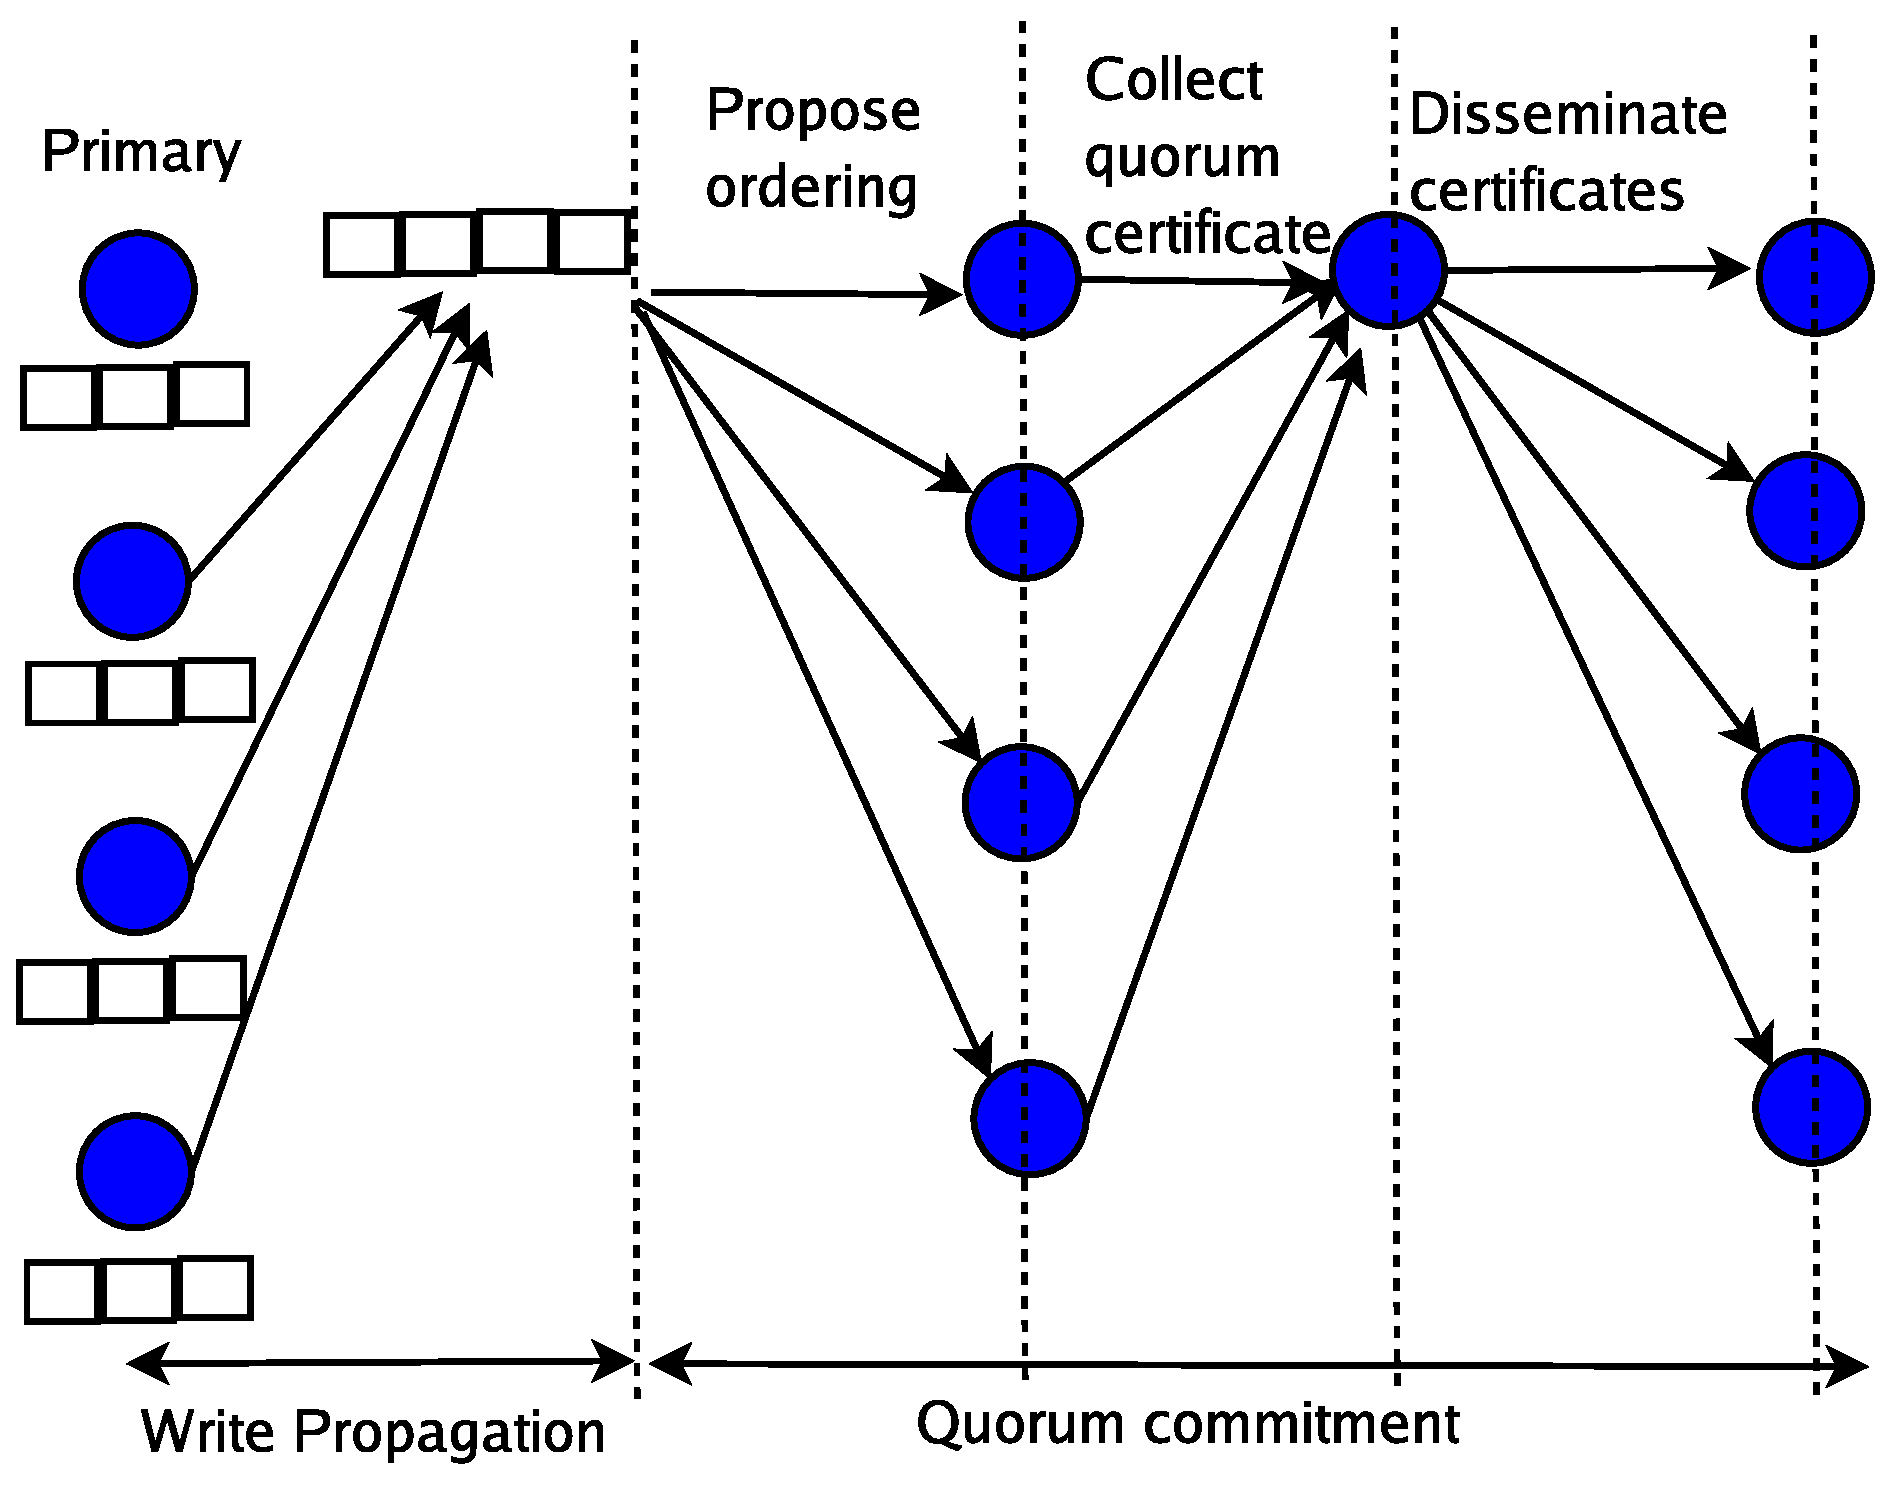
\includegraphics[width=3in]{protocol-diagram.eps}
\caption{Replicas propagate updates to the primary. Primary collects and proposes an ordering. Other replicas check the ordering and if correct they send an ACK. Primary collects a quorum of such ACKs and then disseminates them to the system.
}
\label{fig:protocol-diagram}
\end{figure}

\if 0
\section{Quota enforcement to prevent Email Spam}
\Sys is particularly useful for the quota-based enforcement systems as suggested in 
Section~\ref{sec:applicability}. We use quota enforcement to prevent email spam~\cite{}.


\subsection{Overview}
\paragraph{Architecture}
Each mail server (MS) is a client to the enforcer system. Before sending an email, a MS
obtains a \emph{stamp} from the system and attaches it to the outgoing email. A receipient
MS checks if the stamp is valid. If not, it drops it considering it to be a spam. Else, it
accepts it and forwards to the mail recipients.

Enforcer system consists of $N$ nodes, which are grouped in $k$ groups, each containing 
$3f+1$ nodes, $f$ is set depending on the expected failure rate. Nodes are assumed be
well maintained therefore have low-failure probability and low churn expectation.

Each MS $MS_i$ is mapped to a group $G_i$ via consistent hashing. Set of nodes that are
mapped to a group $G_i$ are called the "clients" to the group, $C_{G_i}$. Note this is a 
\emph{sender-oriented} grouping of the enforcer nodes. One could also group the enforce
nodes based on the receipients. More on the receiver oriented grouping later.

\paragraph{Application state(S)} Each MS is mapped to a record $R$ which logically contains
following fields: (i) $\msg{ID}$, (ii) $\msg{K}$ (public key), (iii) $\msg{T}$ (time period), (iv) $\msg{Sent}$: a variable representing number of emails sent in T so far and (v) 
$\msg{Sent-Th}$: a threshold on number of emails that it can send in T. Note that 
$\msg{Sent-Th}$ can vary across commits but remains constant during a timeperiod T.

How does the conit function $F$ defined? What exactly happens during the commit?

\paragraph{Core algorithm} At a high level, when MS needs to send an email, it sends a request to obtain a stamp from the system. If $\msg{Sent} < \msg{Sent-Th}$, system grants the stamp and sender attaches the stamp to the email. Else, MS is not given the stamp, 
essentially preventing it from sending legitimate email in the current time period. \Sys allows us to implement an approximate version of the above check such that $\msg{Sent} < \msg{Sent-Th} \pm \delta$.



\subsection{Threats and goals}
At a high level, our goals include: spammers are not able to send an order of 
magnitude more email than correct email senders. Zero false positives. 

Tolerate arbitrary number of faulty MSes and bounded number of faults in enforcer
system.

\subsection{Using \Sys}
Each MS gets a quota $q$ of email that it can send in a given time period. For simplicity,
assume $q$ to be same for every MS. We focus on how a group $G_i$ and its clients $C_{G_i}$
function.

\paragraph{Configuring \Sys}
The total number of non-spam emails allowed by $G_{C_i}$ in a given time period is given by $|C_{Gi}|.q$. Per client, the allowed emails per time period is $q$. So, the maximum emails that a faulty client can send in this system is $|C_{G_i}|$, which is $(|C_{G_i}|-1).q$ over the allowed quota. Set $\alpha=(|C_{G_i}|-1).q$, which translates to $\beta=\alpha/|G_i|=(|C_{G_i}|-1).q/(3f+1)$. If $|C_{G_i}|-1> 3f+1$, then error is positive, meaning that "some" client may send more than $q$ quota of emails in a given time period. By setting $\alpha$ to different values, we can bound the maximum emails that a faultly client (an MS) can send.

\subsection{Obtaining a stamp}
Note that the request sent by the clients of the \Sys protocol have the following format:
$<\msg{Req}, o, t, c>_{a_c}$. We now identify what $o$ contains for the spam prevention
application. $o$ contains: (i) cryptograph hash (e.g., SHA-1) of the email-content, 
(ii) hash of the receipient's
email address and (iii) hash of the sender's email address.

Note that we could also put recipient mail server's id in $o$ in plain-text, so that the enforcer system
could use the MAC authenticator instead of the asymmetric key cryptography. However, that
would hurt the privacy (enforcer system knows the identity of the mail servers of both sender and receiver).

Each replica in the group applies the \Sys algorithm and responds as long as the cumulative
number of emails send so far across the clients of the group is less than $\beta$ while the requests are monotonic from each client. The response to a request is prepared by putting the
$o$ in the response so that the recipient verify the integrity of the email, and check if the
stamp was in-fact obtained for the given email. Note that each email is an unit weight 
update to the counter maintained. Also note that once $\beta$ bound is reached, a commit
is done to calculate the precise usage (number of emails sent in last time slot) for each client.

During the commit phase, each client's actual usage is calculated and clients who have
sent more than $q$ number of emails in the last time period are allowed to sent
correspondingly less number of emails in the current time slot.

Once a client (MS) obtains a quorum of $2f+1$ identical responses from the group (called a 
\emph{certificate}), it 
attaches the ceritificate to the outgoing email.

\subsection{Verifying stamp}
If the certificate to an incoming mail is valid, the email is considered authentic and 
forwarded to the mail box of the receipient. Else, it is dropped. Note that verification
is simply verifying $2f+1$ signatures, which is strictly a local operation.

\subsection{Benefits}

\paragraph{Qualitative} (i) No blackmarketting of stamps since stamps are unique to sender, receipient tuple. (ii) Sender is responsible for contacting the enforcer, receiver simply verifies which is a local operation. (iii) No false positives. 
%(iv) We can configure $q$ per receipient mail server, which can be modified online by the receipient. (v) Stamps are not re-usable across receipients.

\paragraph{Quantitative} (i) Need to support current email workloads. (ii) What is the size of enforcer system we need?
\fi

\section{Distributed Online Games}
Here we illustrate the usefulness of \Sys protocol to tackle Byzantine faulty players
in distributed online games. 

\subsection{Background}
System state consists of both mutable and immutable data. Immutable data typically consists
of game map and geometry. Mutable data consists of the player avatars, projectiles (missiles) etc.

Under client server architecture, whole system state is maintained in centralized servers. There
are obvious disadvantages: scalability concerns, performance bottlenecks, large maintenance costs etc.
Distributed gaming architectures are being explored.

In distributed setting, the mutable state is partitioned across participating nodes (p2p architecture).
This part is based on Colyseus, a distributed game being developed at CMU (Srini's group).
Each object is assigned to a node, called its primary. All updates to the object are serialized
through the primary of the object. Other replicas obtain a backup replica of an object by locating
it in the network via some range-queriable DHT (Mercury). Nodes apply updates to local backup 
copy and propagate update deltas at a periodic rate to the primary. Primary serializes them and
then propagates all updates received in the last time slot to every node holding a backup replica
of the object. 

%\begin{table}{c|c|c}
\begin{table*}
\centering
%\begin{tabular}%{1.0\textwidth}{|c|c|c|c|}
\begin{tabular}{|c|c|c|c|}
%\caption{Identifying where different functionalities are located in three architectures for online games.}
%\label{tab:comp_arch}
\hline
Operation types & Client/Server & Everything Distributed (P2P) & Hybrid (ours) \\
\hline
\hline
State & Centralized (@ Server) & Distributed (partitioned across player nodes) & Distributed  \\
\hline
Computation/Execution & Centralized & Distributed & Distributed\\
\hline
Game rule enforcement & Centralized & Distributed & At Enforcement nodes \\
\hline
%Updates & Contact Server & Local & Contact Enforcer system\\
%\hline
%Object location & Contact Server & DHT/Range-query & Contact Enforcer system\\
%\hline
%Security threats & Trusted server. & Deal with cheating, malicious servers. & Trusted Enforcer system. \\
\hline
\end{tabular}
\caption{Identifying where different functionalities are located in three architectures for online games.}
\label{tab:compare_arch}
\end{table*}

Per-object consistency is maintained by the above mentioned primary-backup protocol, where backup
replicas trail the primary by some time window (time to propagate update to primary
and hear back). In addition, each player has a view of the game based on the objects and game
map it is interacting with. This defines the view consistency. Colyseus has two types of view
inconsistency: missing objects in a view and missing/delayed or out-of-order updates to objects. 
Both these inconsistencies can be expressed using TACT model and used by Colyseus. Currently,
Colyseus bounds the \emph{staleness error} while keeping the numerical and order error unbounded.
This is because of the interactability of online games. 

\subsection{Threats}
Colyseus modularizes the system architecture in 3 components: (i) object placement, (ii)
object location and (iii) replica management. Each component is vulnerable to cheating 
players. 

Object placement says which object resides on which nodes. So, if a missile object's primary
resides on a cheating node, then it can manipulate the missile's think function to kill
some other player.

Object location says how to find out the primary for an object. By preventing updates being sent
to other players about its movement, a cheating player can become in-visible.

Replica manager is responsible for serializing updates. If a player's local node is its primary,
then it can order updates in such a way that it is never killed (claim that a "kill" update
is received after it updated its location).

CMU people are currently exploring techniques to \emph{detect} such misbehaviors rather than
\emph{masking} such behavior since masking protocols are too expensive and may break their
interactability requirements.

\subsection{Preliminary design based on \Sys}
We present a solution based on \Sys that masks such misbehavior under specific conditions (defined below).
\if 0
Each object is assigned a replica group, consisting of $3f+1$ nodes. Assignment is done using 
consistent hashing, each node has a $<\{K_{pub/priv}, nodeId\}>$, a key pair 
and a nodeId provided by the gaming company.

Each node is possibly a Byzantine faulty player, a client in BFT terminology. Each node is
also a Byzantine faulty server.

At a high level, each object is both a client and a state variable of the system. It can 
modify some other object (hence state) and also gets modified by some other client. 
\fi
Every update generated in the system should be (i) authenticated, (ii) verified that
it follows game rules and (iii) properly ordered. 


An important observation is that we do not care about the game that a cheating player is
able to see for itself. Rather, our goal is to ensure the non-faulty players see a game play
that adheres to game rules and is approximately consistent. 

\subsubsection{Hybrid Architecture}
We propose a hybrid architecture to combine the benefits of both the centralized system
and a purely distributed system as depicted in Table~\ref{tab:compare_arch}. In the hybrid architecture, the execution and state is distributed at the participating players, however the update ordering and rule enforcement are done at the enforcement nodes. We will discuss how the enforcement system works in a bit. First, we discuss the whole system works.

\paragraph{Architecture} No player node can modify any object directly. It has to go through the enforcement system to get a correct ordering and once it gets that, it can apply locally the updates. This is true for any kind of update, whether it is for updating the location of the own player's game avatar or trying to kill some other player. The additionaly latency is the latency to contact the enforcement system. 

\paragraph{Operation types} At a high level, there are three kinds of operations: object creation, object modification and object deletion. Creation consists of a new player joining the system, missile object being created, health-packs appearing with time. Updates operations include geographic location modification or health modification of a player, motion of a missile in a projectile, action of bots (e.g., computer controlled monsters).




\textbf{Questions that confused me last time:}
\begin{enumerate}
\item{Is RYW (read-your-writes) useful in this application?:} Answer: yes, it is and depends on the conit function defined for the updates that a player can do. For example, if a player is simply roaming around and not interacting with players, then it is sufficient to just see that the player is actually moving. This assumes that small modifications in the location of the player do not weight much. Consider a situation when a player fires a missile at another user. Assuming that creation of missile warrants an immediate commit, at that point, system will become consistent. If missile does not kill the other player, this may simply mean that the other player moved before missile exploded which is valid under linearizability and that is also the best a centralized client/server implementation could afford. So, it all depends on how conit functions are defined.
\item{} Given that Colyseus uses only staleness error, does it make sense to use \Sys at all? Or should
we think about how numerical error can help? Or how do we incorporate staleness in \Sys?
\end{enumerate}

\subsubsection{Enforcement System (ES)}
Our goal is to identify how ES works and how many nodes do we need to scale up to large size online games.

First, nodes in the ES are well maintained, have low failure probability and low churn. They are partitioned in groups of size $3f+1$, assuming that no more than $f$ fails in any group.
Let ES has $N$ nodes and $k$ groups, $k=N/(3f+1)$.

Objects are partitioned over the groups via consistent hashing, $o_i \rightarrow G_i$, where $G_i$ is node whose id is closest to the id obtained by SHA-1 hash of the $o_i$'s id.

\paragraph{Locating objects in a region} Now, the question is how does a player locate which objects it is interacting with in a region? Colyseus uses a range-queriable DHT. We need a reliable and secure way, so probably use ES. 

\paragraph{Propagating updates} There are again two types of updates: updates that affect own state and updates that affect remote objects. 

\paragraph{Defining conits} Each object defines a conit and weights of updates differ for different type of updates. 


\if 0
\section{Invariants}



\subsection{Invariants by consistency protocol}


\textbf{6. Reads by non-faulty clients are always guaranteed to see bounded NE.} \\
\textbf{Proof:} Three cases
to consider depending on earlier writes by the same client.
\begin{itemize}
\item{\textit{No previous writes}} This case is easy to see since at least (f+1) non-faulty replicas will
match in their responses.
\item{\textit{Only admitted writes}} This is also easy to see since admitted updates, by definition,
see bounded NE. Hence, reads which see only admitted writes see bounded NE also. 
\item{\textit{Admitted and submitted writes}} This case is not possible since a non-faulty client
would not send a read request before ensuring that previous write was admitted. This case
holds vacuously.
\end{itemize}

\textbf{7. Submitted writes are given best effort guarantees.} \\
\textbf{Proof:} This follows from our definition
of a submitted update. A submitted update can be received by a slow but 
non-faulty replica who may not participate in the next checkpoint. This may cause
the error bounds to violate. However, if a fast and non-faulty replica receives the
request, it may appear in the next checkpoint and error bounds are preserved. Hence,
it is dependent on how the network delievers requests and since we do not
assume ordered delivery, we can only provide
best effort guarantees unlike the ``admitted'' writes where we ensure that numerical
error guarantees are strictly enforced.\\

\textbf{8. Exactly once semantics.} \\
\textbf{Proof:} Replicas remember the timestamp of last 
executed request for each client and discard requests whose timestamp is lower than that.
This is similar to how BFT provides exactly once semantics.\\

\textbf{9. RYW session guarantees for non-faulty clients.} \\
\textbf{Proof:} Here, W identifies only the 
admitted updates from a given client. We need to prove that if a client
receives (f+1) matching responses, then that result is the non-faulty result. A 
result is non-faulty if is based on the latest checkpoint seen by the system
and has observed the effects of latest admitted updates by a given client not
present in the latest checkpoint.

First note that an admitted update is received by at least (f+1) non-faulty
replicas. From Line 4 and 5 of \texttt{check-response()} in client automaton,
it is clear that a client will wait for (f+1) matching responses but does so after
waiting for (2f+1) responses. This prevents the faulty replicas from providing responses
matching the response from a non-faulty replica who has missed some number of 
checkpoints. By waiting for (2f+1) responses, it is guaranteed that at least 1 non-faulty
replica who participated in the latest checkpoint also responds.  

Since it is possible that f non-faulty may not respond to a client's request,
these might be the ones who participated in the latest checkpoint. Hence, the 
responses may not match (responses match when their CSN is same and there is no more
recent CSN than that). When this happens, a client will retransmit the
request. Given our weak synchrony assumption, sufficient retries will guarantee
that eventually sufficient replicas will respond with same response and same CSN 
and allow the client to make progress.

\textbf{10. If primary is faulty and attempts to reject admitted updates from appearing
in a checkpoint, then view change will be triggered.}\\
\textbf{Proof:} Follows from Invariant 4 where we prove that a checkpoint will
be guaranteed to contain all updates admitted by the system after last checkpoint. At least
(f+1) non-faulty replicas will check for the presence of admitted updates in a proposal and
if not present, these many would initiate a view change. This is sufficient to successfully
complete a view change, from BFT.

\textbf{11. A replica may propagate more than $\beta$ weighted updates during 
a checkpoint but will not violate error bounds for admitted updates.}\\
\textbf{Proof:} Two parts to the proof. First, when primary is non-faulty.
A non-faulty primary will check for the weight of updates propagated by 
a replica at line 2 in function \texttt{check-commit()} and hence will
reject these proposals from committing. A faulty
primary may not check for it and may incorporate these updates in a 
commit message. Again there are two sub-cases. First, incorporating these
'additional' updates from faulty replicas may cause the commit message to 
exceed $\alpha$ weight. This will not be allowed from Invariant 3. Second,
these 'additional' updates from faulty replicas do not cause the $\alpha$
bound to exceed, but at the same time, all admitted updates are present
in the commit message (from Invariant 4). In this case, it does not 
matter whether a faulty replica submitted more than $\beta$ weighted updates
since error bounds for admitted updates are preserved.

\textbf{12. A faulty replica can not initiate commit too early.}\\
\textbf{Proof:} We first define what we mean by too early. If a replica
attempts to commit its tentative updates, we need to ensure that its
tentative log of updates have weight less than or equal to $\beta$. However,
this alone is not sufficient to prevent a faulty replica from attempting 
to commit an update as soon as it receives one. To prevent this from 
happening, line 5 of function \texttt{check-commit()} checks if F(T+$<$o$>$)
exceeds $\beta$ and F(T) $\le \beta$. This ensures that a replica is 
attempting to commit only when needed. So, this is guaranteed when primary
is non-faulty. When primary is faulty, it may itself initiate a commit too early.
However, note that at line 2 of function \texttt{send-updates()}, each 
non-faulty replica checks if the updates in the COMINIT message are
not too early. Only then a non-faulty replica sends its local updates.
Also, a commit is successful only if at least (f+1) non-faulty replicas
participate in it, which is not possible given that no non-faulty replica
will send its updates for such proposals and therefore would fail to find
its updates in the commit proposal. This will prevent a commit from happening.

\textbf{13. (Liveness condition 1) A checkpoint commit is successfully initiated when
\begin{enumerate}
\item{} At least 1 non-faulty replica reaches its bound and primary is non-faulty.
\item{} At least (f+1) non-faulty replicas reach their bound and primary is faulty.
\end{enumerate}
}
\textbf{Proof:} Case 1 is easy to see since a non-faulty primary would initiate a FETCH
of updates from at least f other non-faulty replicas. Once that happens, it would initiate
the BFT protocol to commit the updates contained in the union of these fetched updates.

Consider the situation when primary is faulty. It may not initiate a FETCH 
after it receives a COMINIT message from a non-faulty replica and also 
may not initiate BFT protocol. Our protocol (line 10 of function \texttt{commit-init()})
would require the initiating non-faulty replica to
start view change protocol after sufficient retries. Given that f+1 non-faulty replicas
reach the bound (from Case 2), at least these many would attempt to initiate the view
change. These many are sufficient to successfuly find a new primary and if it non-faulty,
the new primary will initiate BFT's 3-phase commit protocol. 

\textbf{14. Our protocol will deadlock when faulty clients fill up the local buffer of at 
most f non-faulty replica who participated
in the latest checkpoint.}\\
%(b) There are less than $\beta$ non-faulty clients actively submitting updates to the system.
\textbf{Proof:} 
A non-faulty replica responds to client's requests if it has seen all previous requests
from that client and has participated in a recent checkpoint. A faulty client can potentially
send its updates to only a single non-faulty replica (call it R) and fill up its local buffer of $\beta$
updates, causing this replica to initiate commit and stop accepting updates from other clients.
If primary is faulty, it may not initiate the BFT protocol to commit these updates. Replica R may
then initiate a view change, but it will not be successful since not sufficient non-faulty replicas
particiate in it. 

Now let us see how does this affect the non-faulty clients. Recall that a non-faulty client will
retry its updates until they are admitted. However, they will not be admitted since R will not 
respond to these updates and an admitted update needs at least f+1 non-faulty replicas respond. 
Notice now that if we have only one such non-faulty client, it will block waiting for R and R will
block waiting for the view change and no other non-faulty replica will participate in view change.
Hence our protocol will block.

\textbf{15. (Liveness condition 2) A non-faulty client will eventually 
get its request "admitted" and therefore committed as long as at least 
there are 2$\beta$-1 other non-faulty clients actively submitting updates.}\\
%$\beta$-1 other non-faulty clients are actively submitting updates.}\\
\textbf{Proof:} From Invariant 13, as soon as f+1 non-faulty replicas have
their local buffer full (i.e., they have locally seen either $\beta$-weighted positive or negative 
updates), they will 
commit their tentative updates. We need
to show that if there are 2$\beta$ number of non-faulty clients actively
submitting updates, they will eventually fill up the buffers of f+1 non-faulty
replicas who participated in the latest checkpoint and therefore initiate
a commit. To see that, observe that each of these 2$\beta$ non-faulty clients
will be attempting to submit update of absolute weight at least 1. Note that the absolute
weight of all these updates is 2$\beta$ and hence are sufficient to fill up either the 
T$_{+}$ or T$_{-}$  buffer of at least f+1 non-faulty replicas. Now we need to show that as long as
non-faulty clients keep retrying, this will happen eventually.

In the best case,
each of these updates will be ``admitted'' and hence will fill up the local
buffer of f+1 non-faulty replicas. In the worst case, each of these updates
is accepted by at least one non-faulty replica (since it has space in its
local buffer as each can accept upto positive or negative $\beta$-weighted updates) who participated 
in the latest checkpoint. Since non-faulty clients retry until their requests
get admitted, their attempts will eventually fill the buffers of at least f+1 such replicas.

\textbf{16. (Safety condition) An admitted request sees bounded error.}\\
\textbf{Proof:} Follows directly from Invariant 5.
 

\textbf{17. Non-interference with the original BFT protocol execution.}\\
\textbf{Proof:} We want to prove that our consistency
protocol does not interfere with the BFT protocol execution, i.e., once BFT protocol
starts execution, our consistency protocol will not prevent it from completion. 
This is important because we need to ensure that BFT's 
safety and liveness properties regarding checkpoints still hold. To prove that,
we first observe that our modifications to the BFT protocol affect only the 
initiation of the first phase of the BFT execution. Precisely, our protocol
checks for more conditions before accepting a PRE-PREPARE message. We need to show
that these additional conditions do not prevent a valid checkpoint from committing. A 
valid checkpoint is defined as follows: it has sequence number 1 greater than the last
checkpoint's sequence number and contains a set of updates whose weight is bounded by
$\alpha$ and contains all admitted updates. Invariant 1 ensures the first property,
Invariant 3 ensures the second property and Invariant 4 ensures the third property.
Our additional conditions simply check these 3 properties and if they are violated,
at least f+1 non-faulty replicas would initiate a view change. Otherwise, at least these
many would participate in the BFT protocol execution. Hence, our protocol does allow
a valid checkpoint to go through the BFT protocol and allow it to get committed.
Finally, we do not modify any other aspects of the BFT protocol (e.g., handling of
PREPARE, COMMIT messages, view changes) and hence do not interfere with those.
Therefore, once BFT protocol passes the first stage, it will complete its 3-phase
protocol as per the BFT protocol.

\section{Observations}
\paragraph{Configuring BFT} Original BFT allows multiple requests to be 
processed in parallel in the 3-phase protocol to assign them a sequence number.
Our consistency protocol requires some updates to commit and execute before
others to ensure the error bounds are met. This implies that we require BFT
protocol to assign a sequence number to a set of updates before they can 
assign a sequence to next batch of updates. We achieve this by configuring
BFT to have high water mark (H) and low water mark (L) differ by only 1. 
This will provide the desired effect.

\paragraph{View change protocol} There is no modification to the view
change protocol of the original BFT protocol. Replicas may make
more calls to the view change protocol, depending on our algorithms, however
there is no modification.

\paragraph{Modifications to BFT} Our protocol serves as a wrapper protocol
for the BFT protocol. Applications do not directly interact with the BFT.
Instead, they call our protocol's interface and depending on the consistency
requirements, our protocol calls BFT's interface. The only modification to
the BFT protocol execution is the extra conditions being checked at the first
stage (PRE-PREPARE), where non-faulty replicas check for the existence of 
their local tentative updates in the proposal.


\paragraph{Impact of concurrency} 
When multiple clients submit requests to the system, they may get to 
different replicas in different order. This may affect the fraction of
requests which are admitted to the system. Consider a simple setting where
we have a system-wide lock. Each client acquires this lock before submitting
its updates. Other clients block. Under this setting, all requests submitted
to the system are admitted since a non-faulty client will not release
the lock unless it gets an ACK from at least 2f+1 replicas. So, under concurrency
free periods with ordered message delivery, our system will admit every update
submitted by non-faulty clients.

Now, let us illustrate how concurrency might affect the fraction of 
admitted updates. Consider N=4 (r0--r3), f=1 and $\alpha=6$. Under strawman design,
$\beta=2$. Suppose we have 5 clients, c0--c4. Client c0 submits request w0
and gets an ACK from 2f+1 replicas. w0 is now admitted. Now suppose c1 submits
update w1 but gets an ACK from only r0, c2 submits w2 and gets and ACK from
only r1 and c3 submits w3 and gets an ACK from r2. Client c4 submits w4
and gets and ACK from r3 and c5 submits an update w5 and gets an ACK from r3.
At this point, each non-faulty replica is full and tries to commit. Only update
w0 is admitted out of 6 updates submitted to the system W=$<$w0w1w2w3w4w5$>$.
Error bound for w0 is maintained since under any ordering of W, w0 can have
at most 5 updates in front of it. The point to note is that there is only 1 admitted update out
of 6 updates and its error bound is not violated. 

\paragraph{Overhead estimation} In our Strawman design, each request is multicast
to the whole system, each one of them might respond. So, under optimistic
execution, each request will be admitted in 2 message delays. At every $\beta=\alpha/(N-1)$
updates, system will commit updates using consensus, causing O(N$^2$)
overhead. So, the message cost per $\beta$ operations is $\beta*N+N^2$.

For the advanced technique, each request is multicast to the whole
system, wait for 2f+1 ACKs and send these ACKs again to the whole system.
Wait for 2f+1 ACKs. Again, under optimistic execution, each request
will be admitted in 4 message delays. At every $\beta'=2\alpha/3$ updates, system will commit them
using consensus, causing O(N$^2$) overhead. Again, the message cost per
$\beta'$ operations is $\beta'*N+N^2$.

For comparision, each request in original BFT is sent to primary, is processed
through a 3-phase commit and then response is sent. Under optimistic execution,
will take 5 message delays and every $\beta$ operations, the 
message cost is $\beta*N^2$. 

So, the ideal throughput gain is $\beta*N^2/(\beta*N+N^2)=1/(1/N+1/\beta)$.
Setting N=10 and $\beta=5$, we have an ideal throughput gain of factor of 3.
 
\paragraph{Faulty clients}
Other than sending writes at a high frequency so
that the system does consensus more frequently, what can they do? (This is
a DoS attack). Possibly
putting a rate limiting feature can help. Also, faulty clients can not
violate the RYW session guarantees to non-faulty clients.

\paragraph{Faulty replicas colluding with faulty replicas} A faulty replica
can initiate a commit as soon as the faulty client issues that many updates.
Essentially, they may cause commits to happen at a higher frequency and 
probably reduce the benefits of our approach. One defense is to ensure that only
when weight of admitted updates reach a given threshold, then only commits can
happen. This will require faulty clients to send requests to non-faulty replicas,
who can now implement a form of rate limiting to mask this DoS attack.

\subsection{Feedback:}
\begin{enumerate}
\item{} Cleanly separate the consistency protocol and the BFT protocol.
\item{} Latency vs Bandwidth tradeoffs. How does latency of results
in Castro's algo scale with N? What is the interaction between
latency and bandwidth? 
\item{} What if multiple replicas attempt to start the checkpoint at the same time? (Gon)
\item{} Should the system checkpoint as soon as one replica is full? Does it not
degrade the benefits? (Gon)
\item{} Clearly state the distinction from original TACT. (Gon)
\item{} Need to find an application where we understand the semantics of operations and
it is easy to do automatic conflict resolution. (Peter)
\item{} If possible, avoid automatic conflict resolution. (Peter)
\item{} Original BFT protocols do not care to provide guarantees to faulty
clients. However, some applications (micropayments) might need to bound the
behavior of faulty clients. 
\item{} What are the precise limitations of our protocol: we definitely
share the limitations of optimistic consistency protocols (i.e., dealing with
conflict resolution) which limits its usage to applications where it easy to do.
\end{enumerate}

\section{Modified protocol}
We need to handle 3 weaknesses of our protocol:
\begin{enumerate}
\item{} Faulty clients and replicas causing commits to occur at a higher
frequency. Basically we need a rate-limiting feature for clients.
\item{} Reducing the frequency of commits, i.e. have $\beta$ as close as 
possible to $\alpha$.
\item{} Avoid the deadlock problem.
\end{enumerate}

All three problems can be solved by getting feedback from non-faulty clients. 
Intuitively, each non-faulty client waits for its updates to be admitted. Once
that happens (gets f+1 matching responses with latest CSN), it sends these
responses (f+1 signatures) to the system again. Each non-faulty replica keeps
track of the admitted updates and initiates a commit only when the weight of 
the admitted updates has reached $\beta'$ ($\beta'$ is different from $\beta=\alpha/N$).

\fi

\if 0
\section{BFT Clarifications}
Suppose client 1 sent two requests A(1) and B(2). 1 and 2 represent the
timestamp. Now primary may be faulty or due to unordered delivery, it may
receive B(2) first and may assign a sequence number to it and start the 
3-phase protocol. B(2) might commit first than A(1). Since B(2)'s 
timestamp is higher than initial info kept at replicas, they will 
execute B(2). However, when they receive A(1), it will not be executed
since its timestamp is lower and replicas would believe that A(1) was 
executed before. This does not seem right.

-- Response from Rodrigo: This is not an issue since non-faulty clients are
expected to send one request after another.



\section{Applications}

Survey on optimistic replication~\cite{optimistic-repl-survey} gives
a list of wide-area applications which inherently rely on optimistic
replication, such as, DNS, USENET and CVS.

\subsection{Secure Resource Accounting System}
User population denoted as $U$, each user i is represented as $u(i)$. Each
user is assigned a quota of resource q(u(i)) and at any time t, the usage
of quota is represented as p(u(i),t). Goal is to maintain following invariant:
$\forall t |p(u(i),t)-q(u(i))| \le \delta$, where $\delta$ is the tolerance
the application can sustain. $U$ is divided into two components: resource 
consumers (RC) and resource providers (RP). RC and RP could be potentially
overlapping. We also have a potentially separate set of 
enforcer nodes (terminology borrowed from DQE~\cite{Walfish2006}) that maintain the
resource usage account for each user. RC send requests to RP nodes, and 
RP nodes check the quota usage with the enforcer nodes before granting
resource. Both RP and RC could fail either in fail-stop or Byzantine mode.
Enforcer nodes maintain a count for each RC, depicting the quota use for
each RC. Each RP servers as a client which reads/writes these counter values.
RYW property is optional. Depending on the workload, it may not be possible
to use BFT out-of-the-box due to potentially excessive overhead (both 
communication and computation). 

\paragraph{Quota based spam prevention system (DQE [NSDI'06]):} DQE 
avoids relying on BFT by indirectly enforcing a bound on quota usage by
probabilistically preventing stamp re-use. Stamp quota is divided into
individual stamps and enforcer nodes store the stamps they have seen for 
a limited duration. By storing immutable data (hash of stamps), they avoid
requiring replicas to be consistent. However, the price paid is the storage
of large amount of stamps, making disk seek the bottleneck resource. Moreover,
there is no locality in the disk accesses since hashes are random. Another
important observation is that network overhead (quering a small set of 
enforcer nodes for a given stamp) is not a bottleneck (few Mbps). 

Our approach
provides a different point in the design space. We represent the quota usage
of each mailserver by a \textit{single} integer, though it is mutable and 
requires BFT for replica consistency. This avoids the storage as a bottleneck.
Moreover, keeping numerical error sufficiently high would avoid BFT protocol
overhead to be excessive (which is reasonable assumption since our goal is to
prevent large scale spamming). Each mailserver is hashed to a small subset of
enforcer nodes who maintain the count for its stamp usage and they run our
BIC-BFT algorithm. Note that BIC-BFT allows locality of accesses and allow
the protocol to execute without making excessive disk seeks. Finally, even if
a BFT group has more than 1/3rd faulty replicas, this is not a big problem since
our goal is to avoid large scale spamming (similar arguement to DQE). Moreover,
note that the enforcer nodes are well chosen nodes and hence the probability
of a node failing is quite low, e.g. 0.1 (similar to DQE). Our hope
is that we can reduce the number of enforcer nodes required originally by DQE.
 
\textbf{Challenge} Note that since we are maintaining a count, we need to 
ensure that a single
update is not counted twice. Otherwise, a faulty recipient mailserver could
use one stamp sent by a non-faulty mailserver to update the quota usage 
multiple times to overshoot the quota usage of a non-faulty mailserver. 
We therefore require exactly once semantics and recall that our protocol 
ensures that already. But at the same time, if a faulty
mail server reuses its stamps, it should be counted toward its quota usage.
So, we have two conflicting requirements.

\textbf{Other example applications:}
\begin{enumerate}
\item{} Capabilities based DDoS preventation system (SIGCOMM'05).
\item{} Micropayment systems (PPay'CCS03)
\item{} Quota enforcement in online email systems (Gmail, Yahoo E-mail) or storage
quota enforcement in distributed storage systems.
\item{} Network monitoring.
\end{enumerate}
\fi

\section{Evaluation}

An abstract application where multiple clients updating a counter variable
maintained by the system. Application configures BIC-BFT with varying value of
numerical error (NE) it can tolerate. 

\paragraph{Workload} Varying the fraction of reads/writes. Other than when
committing via BFT, the latency of both reads/writes should be similar under
our protocol (should finish in single round trip).


\paragraph{Dimensions} We need to evaluate our protocol in 2 dimensions with
varying NE in each:\\
(i) scale of the replica group, (ii) rate of operations submitted to the system.

\paragraph{Experiment 1: Microbenchmarks} Compare the read/write latency of operations
with the original BFT implementation. No scaling of replica group. 
Configuration: f=1 for 4 machines. No concurrency - single client is submitting
updates. Expected result: as NE is relaxed, read/write latency of BIC-BFT reduces
linearly. We expect that under normal conditions (when NE is not violated), each operation
(read/write) is finished in single round trip. The interesting question is what
happens when NE is quite low, do we do worse than BFT or equivalent. [We can cut
through our protocol to do BFT directly under low values of NE so that our overhead
is never worse than BFT].

Figure 1~\ref{fig:latency-no-concurrency} will show how the latency scales with increasing NE as compared to the 
old BFT in our local testbed. Same with different types of workloads.

\begin{figure}
\centering
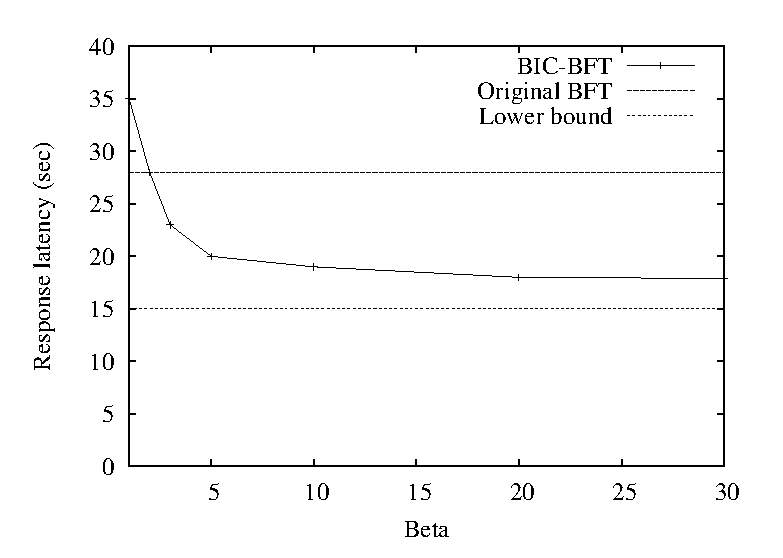
\includegraphics[width=3.5in]{Figures/Latency-50k-1client.ps}
\caption{Response latency averaged over 50,000 requests and 3 runs.}
\label{fig:latency-no-concurrency}
\end{figure}


Draw conclusion about what kind of workloads benefit the most.

\paragraph{Experiment 2: Scaling replica group} Scale N. With different values of NE, see
how the latency scales. Given that as N scales, the cost of consensus increases
quadratically, the benefit of our approach will proportionally increase. 
One caveat is that with same NE (alpha), local beta (beta=alpha/N) decreases with increasing N, 
hence as NE is kept constant and N is increaesed, throughput will drop.

Figure 2 shows how does the BFT scale (response latency) with increasing replica group and compares
how different values of NE provide improvement over BFT. Additionally, it tells
us how our protocol scales with increasing replica group size. 

Figure 3 shows the performance of our protocol with different replica group size and
varying NE. Should see that as replica group is increased and NE is kept constant, our
throughput drop is also linear (since we need to do BFT at higher frequency given beta
increases with N). 

\paragraph{Experiment 3: Throughput} Incorporate concurrency. 
Variable number of clients sending updates to the system, updating the same 
data variable. Vary N with varying NE. This is essentially looking at the
how many requests could be satisfied in a given time period rather than the response
latency as observed in previous figures.

Figure 4 shows how many requests are satisfied as we vary N and NE.


\paragraph{Conclusions we need to draw:}
(i) Overhead improvement linear with respect to the flexibility provided by the application.\\
(ii) Never worse than original BFT.\\
(iii) High throughput.\\
(iv) Better response time.\\

\section{Related work}
1. Work on replicated databases::
 (To name a few related papers:
 Bounded ignorance in replicated systems,
 Sacrificing serializability to attain high availability, Specifying graceful
 degradation in distributed systems etc.)\\ 
2. TACT, PRACTI::\\
3. Consensus style BFT\\
4. Quorum style BFT \\
5. SUNDR:: ensure that untrusted servers can not convince a 
 client to accept arbitrary data, though fork consistency is 
 undetected. Uses public keys and secure histories.\\
6. BFI::
 Isolates the byzantine faults to only parts affected by it.
 Used in Farsite. Partitions the workload in smaller groups to improve
 the throughput.\\
7. OceanStore::
 uses a small set of primary nodes who perform the
 original BFT. Others are secondary replica's, and use epidemic style
 dissemination to propagate the serial order decided by the primary 
 replica's.\\
8. HQ Replication~\cite{hq-replication-osdi-06}: At a high level, HQ exploits 
concurrency free periods to execute requests optimistically 
to avoid the costly server-to-server communication. Reads complete in 1
round trip (1 phase) while writes complete in 2 round trips (2 phases) under 
concurrency free periods. Clients submit updates to the whole system, wait for 
a quorum of 2f+1 replicas. Replicas respond with the sequence number they 
will assign to a given request in phase 1. Once a client receives a quorum 
of matching responses (these many assign the same sequence number),
it resubmits the certificate to the system again (2nd phase) asking them to 
execute the request. A replica would execute the request if 2nd phase 
request contains a quorum of agreeing certificates from phase 1. Under 
concurrency free periods, this will be the case and the update will be 
successful. If there are conflicting updates for a given sequence number, a 
client would notice it in the response to the phase 1 and would request the 
replicas to resolve the conflict by running the original BFT protocol. 

Another important observation made is that at higher scale, BFT induces higher
traffic per request due to use of authenticators (vector of MACs) which were
broadcast to all replicas using a single OS call. Authors show that by 
leveraging MACs and having a TCP connection rather than UDP, they reduce the BFT 
overhead significantly. Moreover, use of preferred quorums reduce the 
overhead even more. 

-- Other uses of relaxed consistency:
-- approximate membership checks to approximate state machines [sigcomm'06]
-- sigmod'06 relaxed consistency for caches


\section{Conclusion}

What lesson did we learn by this?

\bibliographystyle{abbrv}
\bibliography{bft-scale}



%%%%%%%%%%%%%%%%%%%%

\if 0
\subsection{Network File System (NFS)}
[Note: We are trying NFS so as to have apples-to-apples comparision
with previous work. If inconsistency definitions turn out to be 
non-intuitive, we might nuke it.]

\paragraph{Setting} A set of clients access a file system via network.
Whole file system is replicated on N nodes, and f could fail simultaneously.
We assume FARSITE~\cite{FARSITE} style break down of system. BFT protocol
is used to enforce consistency of namespace (metadata) operations. We assume a single
group of N nodes to maintain the full system, rather than partition it
among smaller groups (we will tackle this later). Separate servers
are used to replicate the raw data, system will work as long as at least
1 such server is alive. These servers may not participate in BFT protocol.
Correct clients see RYW.

\subsubsection{Inconsistency tolerated} 
Now, we need to identify what does NE and OE mean under NFS? Turns out
that there are several variants of NE that one could imagine. We illustrate
a few. Basically, we follow the intuitive definition of NE, which says
how far the observed history is from the ideal history. We are trying
to identify meaningful functions to quantify this distance.

Metadata operations in NFS v3~\cite{}: (i) \texttt{getattr}, (ii) \texttt{lookup}, 
(iii) \texttt{readlink}, (iv) \texttt{readdir}, (v) \texttt{setattr},
(vi) \texttt{create}, (vii) \texttt{link}, (viii) \texttt{unlink} and
(ix) \texttt{rename}. First 4 are read-only operations while others
are modification operations.

We partition meta-data operations in two parts: (a) modifying an existing directory
entry (change in file size, modification time etc.) and
(b) creating/deleting an entry in a directory (possibly a directory or a file).
\texttt{getattr} is the only read-only operations, others update the metadata
(even when a user reads a file).
[Need to read in more detail which operation falls in (a) and (b) category.]

\paragraph{Number of meta data operations} In this example, NE
may imply the bounded \textit{number} of meta data operations (both types) that could occur
in the whole system before they are visible to every client. Here, meta
data operations are the operations performed by the clients. Additionally, one policy might be
to have NE=0 for operations performed by administrators (meta-data 
operations in the priviliged part of the system). Since these operations are expected
to be quite in-frequent, we will still have benefits by our approach. 

\paragraph{Amount of data change} Here, meta data operations of type (b) have NE=0, 
while inconsistency is tolerated for type (a) operations. Moreover, the \textit{amount} of 
modification (diff in file size in bytes) counts toward the NE. 

A hybrid policy might make more sense.

\subsection{Network Monitoring}
\paragraph{Setting} A set of firewalls in an enterprise setting monitoring
incoming traffic. Goal is to try to identify if an outside host is sending
too much traffic and if so, raise an alarm. Each firewall keeps track of
a count of how many packets it saw from a given host. Ultimately, this information
is aggregated to evaluate global count of incoming traffic from outside hosts.
A related work is here~\cite{sruti-2005}.

\paragraph{Fault model} Certain fraction of firewalls may fail. These replicas
may not propagate the packets they have seen and these packets may
not arrive at other firewalls also. So, some fraction of attack traffic may go
un-noticed. Questions: can faulty firewalls fabricate packets? Can they
implicate non-faulty hosts? Also, need to clarify what kind of filtering do firewalls
do. 


\paragraph{Inconsistency tolerated} Again, we attempt to identify the meaning
of NE and OE under this setting. Intuitively, NE implies how many updates to the
global counter a particular firewall is missing. This amounts to the rate of
false positive/negative alarms raised by individual firewalls. OE does not matter
here since the only operation applied to the global variable is an \textit{increment}.
Each firewall locally monitors the updates and when they reach a bound, global
commit is done via BFT. One interesting subtle difference with other weak consistency
definitions is that in this setting, replicas may not converge to one consistent
state. This is precisely because certain updates could be visible only to the 
faulty replicas who may not propagate these updates to other non-faulty replicas.
However, this is still useful since we are able to put a bound on these unseen
updates.

\subsection{Revision Control Systems}
This application might make more sense.

\section{Applications}
- online services (airline reservation, banking)

- network monitoring

- file system (AFS, Ivy)

- churn handling 
\section{Other inconsistency definitions}
We study how we can transform the consistency metrics of TACT to 
consistency definitions proposed by others. Here, we list some:
\begin{itemize}
\item{\textit{File system based}} Bayou's definitions
\item{\textit{Calender/mail system based}} 
\end{itemize}
\fi





\end{document}
